\documentclass[a4paper]{jreport}	% 日本語の場合

\usepackage{masterThesisJa-Ja}
\usepackage[dvipdfmx]{graphicx}
\usepackage{hyperref}
\usepackage{breakurl}
\pagestyle{empty}
\usepackage{newtxtext,newtxmath}
\usepackage{algpseudocode}
\usepackage{algorithm}
\usepackage{array}

\setcounter{tocdepth}{3}
\setcounter{page}{-1}


%TODO: 学会ならもっとplotは疎にする、あるいは綺麗なデータをとる
%TODO: 関連研究もっと増やす
%TODO: abort ratioについてのレポート これはYCSB-A,Bにおいて記録しようか それで、スレッド数が増えてもそんなに問題ないことを確認する。データ件数も増やした検証をすべきか?

% 【必須】主題:\maintatile{日本語}{英語}
\maintitle{並行性制御法におけるROS TFの高品質化}{Make ROS TF high quality in concurrency control method}

% 【任意】副題:\subtitle{日本語}{英語}
% 副題が不要な場合は次の行をコメントアウトしてください
%\subtitle{}{}

% 【必須】発表年月:\publish{年}{月}
\publish{2022}{1}

% 【必須】学生情報:\student{学籍番号/CNSアカウント}{氏名(日本語:氏名の間は1文字空ける)}{氏名(英語:Twins登録の表記)}
\student{71970013 / t19501yo}{荻原 湧志}{Yushi Ogiwara}

% 【必須】概要:\abst{概要}
\abst{
 Robot Operating System(ROS)はロボットソフトウェア用のミドルウェアソフトプラットフォームであり、近年多くの研究用ロボットで用いられている。TFライブラリはROSで頻繁に使用されるパッケージであり、ロボットシステム内の座標変換を追跡し、データを変換する標準的な方法を提供するために設計されたものである。ROSの開発初期には複数の座標変換の管理が開発者共通の悩みの種であると認識されていた。このタスクは複雑なために、開発者がデータに不適切な変換を適用した場合にバグが発生しやすい場所となっていた。また、この問題は異なる座標系同士の変換に関する情報が分散していることが多いことが課題となっていた。そこで、TFライブラリは各座標系間の変換を有向森構造として管理し、効率的な座標変換情報の登録、座標変換の計算を可能にした。  


しかしながら、この有向森構造には非効率な並行性制御によりアクセスするスレッドが増えるに従ってパフォーマンスが低下する問題、及び座標変換の計算時に最新のデータを参照することができないという問題があることがわかった。そこで、我々はデータベースのトランザクション技術における細粒度ロッキング法、及び並行性制御のアルゴリズムの一種である2PLを応用することにより、この問題を解決した。提案手法では既存手法と比べ最大455倍のスループットを出すことを示した。
}

% 【必須】研究指導教員(氏名の間は1文字空ける):\advisors{主研究指導教員}{副研究指導教員}
%\advisors{川島 英之}{}
\advisors{川島 英之}


% 以下,本文を出力
\begin{document}

\makecover

\addtolength{\textheight}{-5mm}	% 本文の下限を5mm上昇
\setlength{\footskip}{15mm}	% フッタの高さを15mmに設定
\fontsize{11pt}{15pt}\selectfont

% 目次・表目次を出力
\pagebreak\setcounter{page}{1}
\pagenumbering{roman} % I, II, III, IV
\pagestyle{plain}
\tableofcontents
\listoffigures

% 本文
\parindent=1zw	% インデントを1文字分に設定
\pagebreak\setcounter{page}{1}
\pagenumbering{arabic} % 1,2,3
\pagestyle{plain}

% 章:\chapter{}
% 節:\section{}
% 項:\subsection{}

% 図表:
% \begin{figure}[h]
% \centering
% \begin{center}
% \includegraphics[width=10cm]{fig/<file name>}
% \caption{ <図の一言説明> }\label{fig001}
% \end{center}
% \end{figure}


\chapter{はじめに}
% プレースホルダ
\section{研究背景}

% 質問をここに書く
% abstractでは\citeは使わない
% 起承転結が二つだといいのかな
%TODO 原文から引用しても良いのか?
% ~の問題がある、は適切な表現ではない。lookupTransformについては既存のIFに問題があるわけではない
% 座標変換、座標系といった言葉が冒頭では冗長である。
% 「高精度なロボットにはデータベースの技術が必要だ!!!!」

% ここもTFの冒頭からコピー
ロボットを使って作業を行う場合、ロボット自身がどこにいるのか、ロボットにはどこにどんなセンサーがついており、また周りの環境のどこにどんなものがあるかをシステムが把握することが重要である。例えば、図\ref{fig:room} のように部屋の中にロボットと、ロボットから観測できる二つの物体があるケースを考える。図中にてロボットは円形、物体は星形で表現され、ロボットが向いている方向は円の中心から円の弧へつながる直線の方向で表される。途中で交わる二つの矢印は各座標系の位置と原点、姿勢を表す。ここでは、地図座標系、ロボットの座標系、二つの物体それぞれの座標系が示されている。

システムはロボットに搭載されたセンサーからのデータを元に各座標系間の位置関係を随時更新する。この位置関係は並行移動成分と回転成分で表現できる。例えば、自己位置推定プログラムはLiDARから点群データが送られてくるたびにそれを地図データと比較して自己位置を計算し、ロボットが地図座標系にてどの座標に位置するか、ロボットがどの方向を向いているかといった、地図座標系からロボット座標系への位置関係を更新する。物体認識プログラムはカメラからの画像データが送られてくるたびに画像中の物体の位置を計算し、ロボット座標系から物体座標系への位置関係を更新する。

このように、各座標系間の位置関係の更新にはそれぞれ異なるセンサー、プログラムが使われる。各センサーの計測周期、及び各プログラムの制御周期は異なるため、各座標系間の位置関係の更新頻度も異なるものとなる。図\ref{fig:sensor-sync}では、地図座標系からロボット座標系への位置関係データと、ロボット座標系から物体座標系への位置関係データがそれぞれ異なるタイミングで登録されていることを示している。



\begin{figure}[h] 
\centering{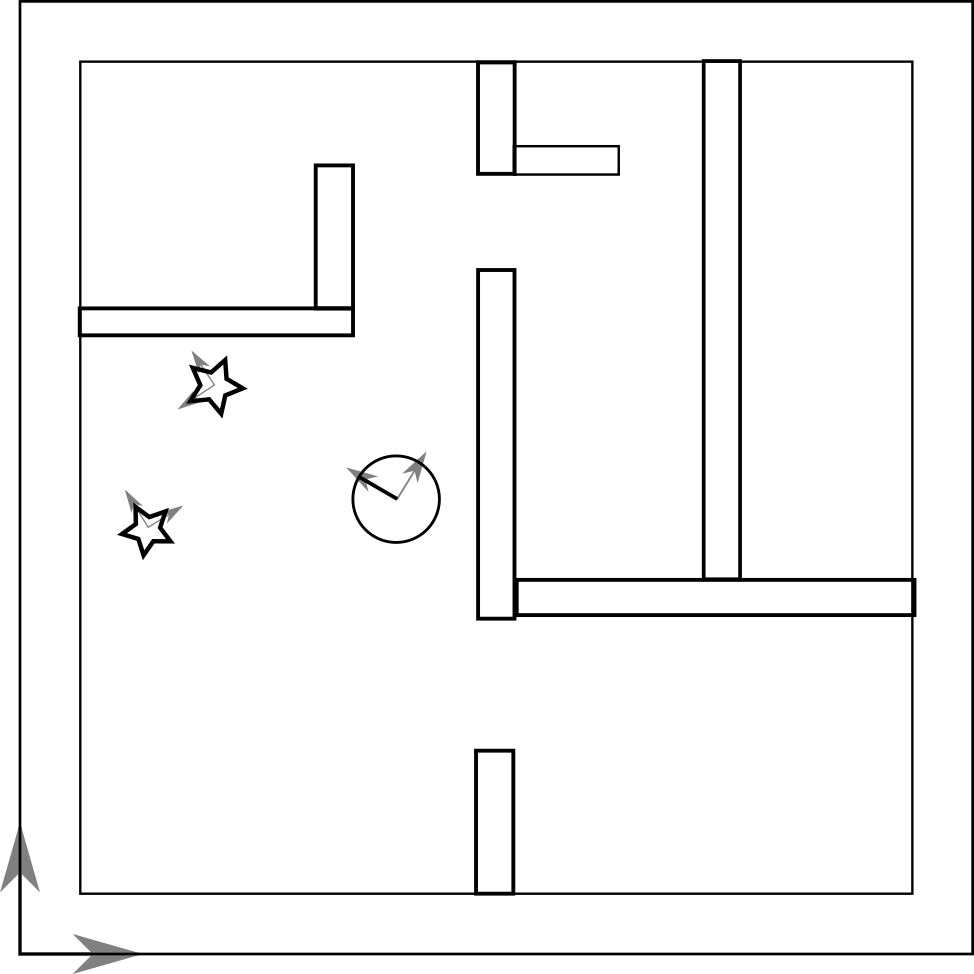
\includegraphics[width=8cm]{room}}	
\caption{部屋の中のロボット}
\label{fig:room}
\end{figure}

\begin{figure}[h] 
\centering{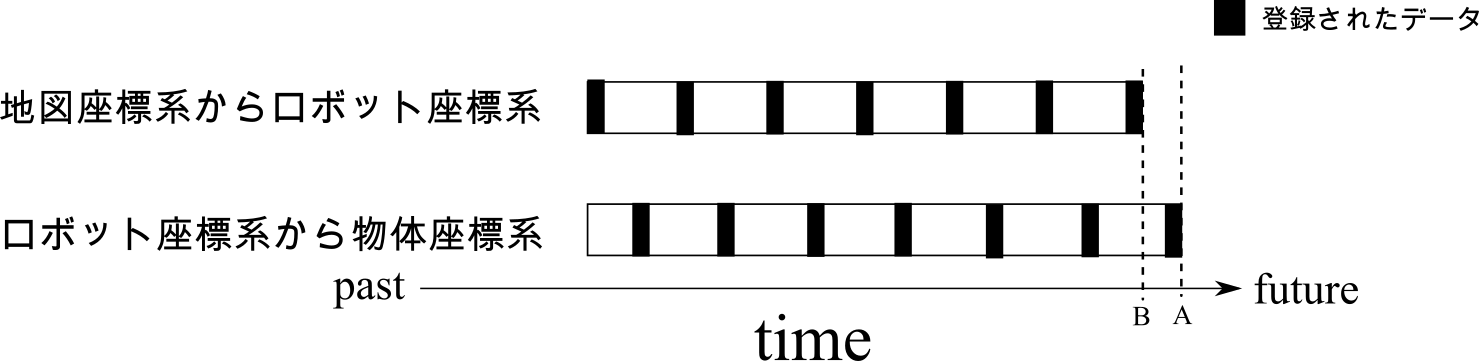
\includegraphics[width=12cm]{sensor-sync}}	
\caption{位置関係の登録のタイムライン}
\label{fig:sensor-sync}
\end{figure}


ここで地図中での物体の位置を把握するために、地図座標系から物体座標系への位置関係を取得する方法について考える。地図座標系から物体座標系への位置関係は地図座標系からロボット座標系への変換とロボット座標系から物体座標系への変換を掛け合わせれば計算ができるが、図\ref{fig:sensor-sync}のように各変換データは異なるタイミングで来るため、最新の変換データを取得するプログラムは複雑なものとなる。Aの時刻で地図座標系から物体座標系への変換データを計算しようとするとロボット座標系から物体座標系への最新の変換データを取得できるが、地図座標系からロボット座標系への変換データはまだ取得できない。このため、最新の変換データ$\theta$を取得する、もしくは過去のデータを元にデータの補外をする必要がある。Bの時刻で地図座標系から物体座標系への変換データを計算しようとすると地図座標系からロボット座標系への最新の変換データを取得できるが、ロボット座標系から物体座標系への変換データはその時間には提供されていない。このため、$\alpha$と$\beta$のデータから線形補間を行う、もしくは最新の変換データ$\beta$を取得する必要がある。
また、地図座標系からロボット座標系への位置関係、ロボット座標系から物体座標系への位置関係はそれぞれ別のプログラムで計算されているため、座標系同士の位置関係に関する情報は分散した状態となっている。


このように、ROSの開発初期には複数の座標変換の管理が開発者共通の悩みの種であると認識されていた。このタスクは複雑なために、開発者がデータに不適切な変換を適用した場合にバグが発生しやすい場所となっていた。また、この問題は異なる座標系同士の変換に関する情報が分散していることが多いことが課題となっていた。

そこで、TFライブラリは各座標系間の変換を有向森構造として一元管理し、効率的な座標系間の変換情報の登録、座標系間の変換の計算を可能にした。まず、図\ref{fig:room}を表す木構造は図\ref{fig:room-tree}で表現できる。木構造のノードが各座標系を表し、木構造のエッジは子ノードから親ノードへの変換データが存在することを表す。
% camera1, camera2の説明はいるだろうか?

\begin{figure}[h] 
\centering
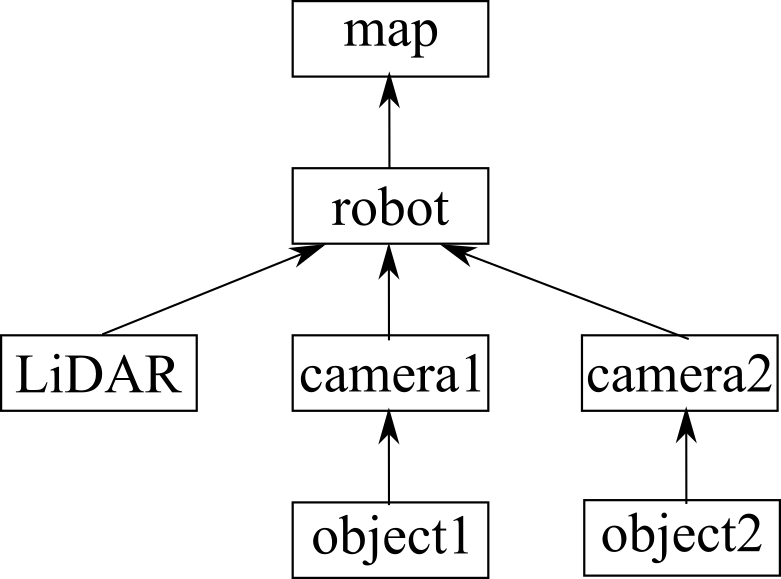
\includegraphics[width=5cm]{tree}	
\caption{図\ref{fig:room}に対応する木構造}
\label{fig:room-tree}
\end{figure}

各ノードはTFではフレームと呼ばれ、ノード中の文字列は各座標系に対応するフレーム名が書かれている。図\ref{fig:room-tree}では地図座標系のフレーム名はmap、ロボット座標系のフレーム名はrobot、物体1の座標系のフレーム名はobject1となる。子ノードから親ノードへ張られた有向エッジは子ノードから親ノードへポインタが貼られていることを表し、子ノードから親ノードを辿ることができる。このため、mapからobject1への座標変換を計算するにはobject1からmapへの座標変換の計算をし、その逆変換を取る必要がある。

子ノードから親ノードへの位置関係情報は子ノード自身が保持する。

先程説明したように、各フレーム間の座標変換情報はそれぞれ異なるタイミングで登録される。これに対処するため、TFでは各フレーム間の座標変換情報を過去一定期間保存する。図\ref{fig:room-tree}において各フレーム間の座標変換情報が登録されたタイミングを表すのが図\ref{fig:room-timeline}である。横軸は時間軸を表し、左側が過去、右側が最新の時刻を表す。黒色のセルはデータがその時刻にデータが登録されたことを表す。時刻Aではrobotからmapへの座標変換の情報が得られるが、object1からrobotへの座標変換の情報は時刻Aには存在しない。そこで、TFでは前後のデータから線形補間を行うことにより該当する時刻の座標変換データを計算する。つまり、TFは該当する時刻の座標変換データが保存されている、もしくは前後の値を元に線形補間ができる場合にはその時刻の座標変換データを提供できる、とみなす。灰色の領域は線形補間により座標変換データが提供可能な時間領域を表す。

\begin{figure}[h] 
\centering
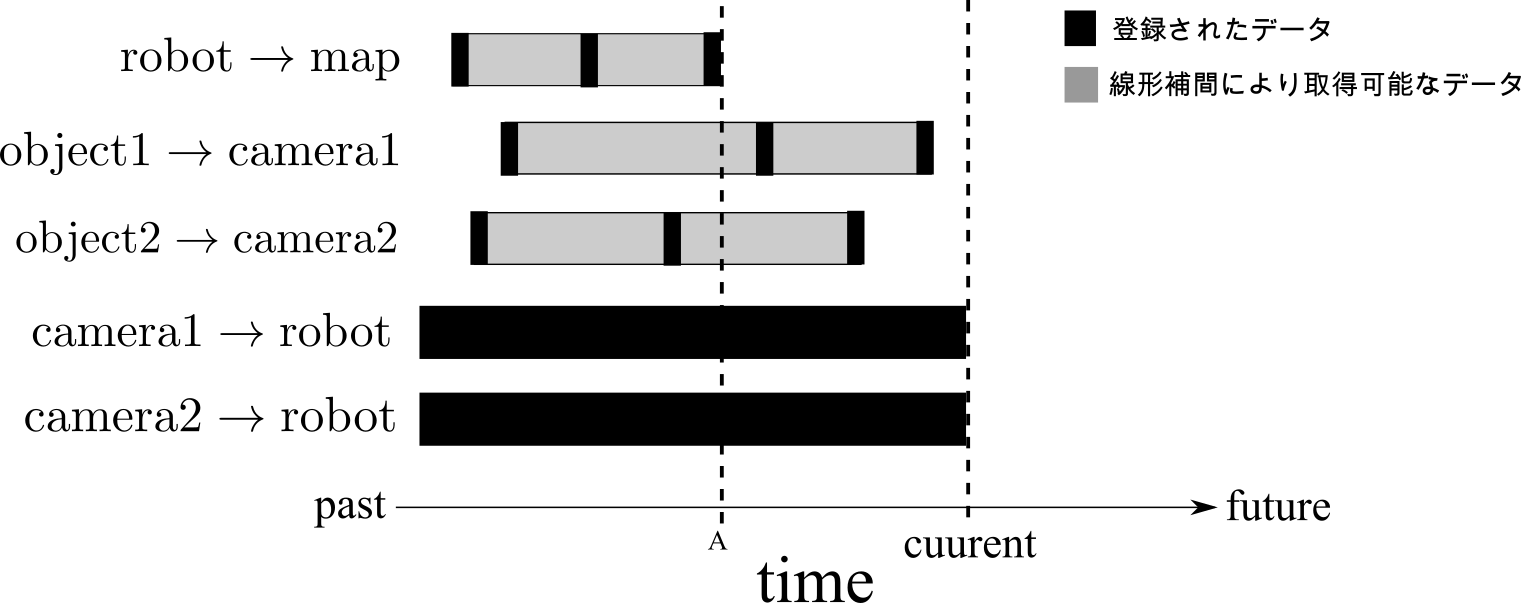
\includegraphics[width=10cm]{room-timeline}	
\caption{図\ref{fig:room-tree}における位置関係登録のタイムライン}
\label{fig:room-timeline}
\end{figure}

図\ref{fig:room-tree}における位置関係登録のタイムラインが図\ref{fig:room-timeline}のようになっているとき、TFではobject1からmapへの最新の位置関係は次のように計算する。

まず、object1からmapへのパスを確認する。ここではobject1からmapへのパスはobject1$\rightarrow$robot, robot$\rightarrow$mapであることがわかる。

次に、どのパスにおいてもなるべく最新の座標変換を提供できる時刻を確認する。図\ref{fig:room-timeline}を確認すると、object1$\rightarrow$robot、robot$\rightarrow$mapにおいて最新の座標変換情報が登録された時刻が最も古いのはrobot$\rightarrow$mapである。このため、時刻Aがここでは要件を満たす。

最後に、時刻Aでの各パスのデータを取得し、それらを掛け合わせる。robot$\rightarrow$mapについては登録されたデータを使い、object1$\rightarrow$robotについては線形補間によってデータを取得する。

\section{研究課題}
前述したようにTFはロボットシステム内部の座標系間の位置関係を一元管理する機構を提供する。しかしながら、これには以下のような問題点が挙げられる。

\subsection*{問題1:ジャイアント・ロック}
TFの森構造には複数のスレッドがアクセスするため並行性制御が必要となるが、既存のTFでは一つのスレッドが森構造にアクセスしている際は他のスレッドは森構造にアクセスできないアルゴリズムとなっており、これは、マルチコアが常識となっている現代では大きな問題となる。

\subsection*{問題2:データの鮮度}

上記の説明のように、TFのフレーム間の座標変換計算インターフェースは最新のデータを使わない可能性がある。同時刻のデータを元に座標変換を行うためデータの同期性はあるが、最新の座標変換データを使わないためデータの鮮度は失われる。現在、TFライブラリには最新の座標変換データをもとにフレーム間の座標変換計算をするインターフェイスは無い。

\section{研究方針}
前述した問題1については、データベースの並行性制御技術における細粒度ロッキング法を適用して解決する。細粒度ロッキング法は、並行性制御においてロックするデータの単位をなるべく小さくし、並行性を向上させる手法である。

問題2については、データベースのトランザクション技術における2PLを適用し、複数の座標変換の最新のデータをatomicに取得するインターフェース、及び複数の座標変換の最新のデータをatomicに更新するインターフェースを提供する。2PLとは、複数のデータに対するロック・アンロックのタイミングを二つのフェーズに分けることにより並行性を向上させつつデータ操作の一貫性を確保する手法である。

\section{貢献}

本研究ではデータベースのトランザクション技術における再粒度ロッキング法、及び並行性制アルゴリズムの一種である2PLを応用することにより、問題1および問題2を解決した。

\section{構成}
本論文の構成は次の通りである。第二章では関連研究について述べる。第三章では既存のTFの森構造とその問題点について述べる。第四章では提案手法である森構造への再粒度ロックの導入とデータ一貫性のためのインターフェイスの提供について述べる。第五章では提案手法の評価結果を述べる。第六章では本研究の結論を述べる。第七章では今後の課題について述べる。

\chapter{関連研究}

データベース分野におけるロボットの研究の例としてはGAIA platform\cite{gaia}が挙げられる。GAIA platformはリレーショナルデータベースと、そのデータベースに変更が加えられた時の処理をC++で宣言的に記述できる仕組みを組み合わせることにより、イベントドリブンなフレームワークでロボットや自動運転システムを構築するものである。
% PostgreSQLのtriggerとはちょっと違う

%TODO SSMはどこから引用すればいい??
% 移動ロボット用センサ情報処理ミドルウェアの開発 か?
TFライブラリのようにデータを時系列的に管理するライブラリとしてSSMが挙げられる。SSMでは各種センサデータを共有メモリ上のリングバッファで管理することにより、時刻の同期を取れたデータを高速に取得することができる。

% 移動ロボット用センサ情報処理ミドルウェアの開発 か?

ROSはロボットソフトウェア用のミドルウェアソフトプラットフォームであり、近年多くの研究用ロボットで用いられている。産業用途にも利用可能にするためにROSの次世代バージョンであるROS2\cite{ros2}の開発が進んでいるが、並行性制御アルゴリズムはROSから変わっておらず、本研究のようなアプローチはない。

データベース分野における高速並行性研究におけるトランザクション処理システムとして2PL、Silo、Cicadaが挙げられる。従来のトランザクション処理システムはハードウェアのコア数が少なく、メモリが小さい中でいかに効率的に処理を行うかに重きが置かれてきたため、2PLなどの悲観的ロッキング法が主に使われていた。
しかしながら、近年のハードウェアはメニーコア化と大容量メモリが前提のシステムとなっており、従来手法では必ずしも性能が最大限出るとは言えない。そこでSilo\cite{silo}やCicada\cite{Cicada}などの楽観的並行性制御法が提案された。これらは近年のハードウェアを前提に設計されているため、それまでのシステムと比べ非常に高い性能を実現する。

\chapter{既存のTFの森構造とその問題点}
\section{構造}
TFライブラリでは図\ref{fig:multitree} のように各座標系間の位置関係を森構造で管理し、複数の木の登録が登録できる。ノードが各座標系を表し、エッジは子ノードから親ノードへの座標変換データが存在し、また子ノードから親ノードへポインタが貼られていることを表す。このため子ノードから親ノードへ辿ることはできるが、親ノードから子ノードを辿ることはできない。各ノードはフレームと呼ばれ、ノード内の文字列は各座標系に対応するフレーム名が書かれている。

各フレーム間の座標変換情報は過去10秒間保存される。このため、各フレーム間の座標変換情報が登録された時刻を図\ref{fig:general-timeline}のようなタイムラインで表現できる。黒のセルは登録されたデータを表し、灰色のセルは線形補間により座標変換データが取得可能な時刻を表す。横軸が時間軸を表し、左側が過去、右側が最新の時刻を表す。

\begin{figure}[h] 
\centering
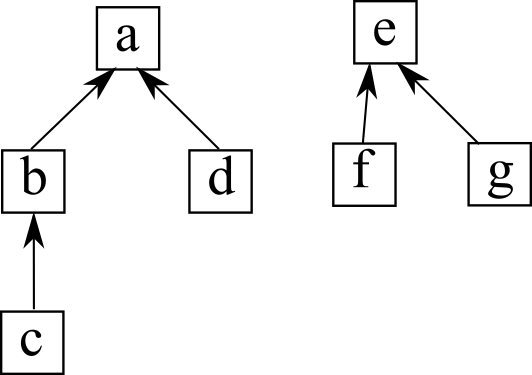
\includegraphics[width=7cm]{multitree.png}	
\caption{複数の木構造}
\label{fig:multitree}
\end{figure}

\begin{figure}[h] 
\centering
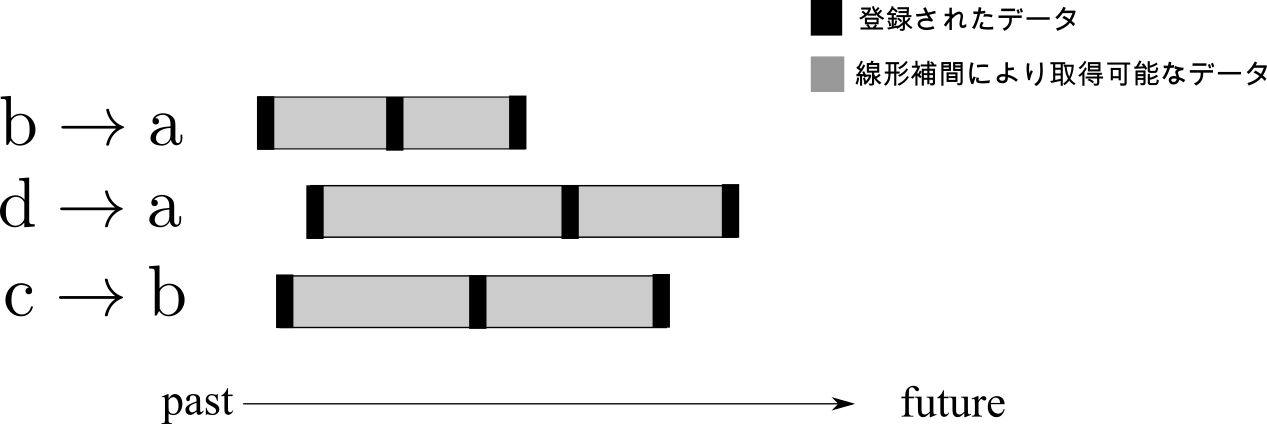
\includegraphics[width=15cm]{general-timeline.png}
\caption{タイムライン}
\label{fig:general-timeline}
\end{figure}


\section{lookupTransform}
二つのフレーム間の座標変換情報を取得するにはlookupTransformメソッドを使う。二つのフレームが同じ木構造に属している場合にのみフレーム間の座標変換が計算できる。

% need algorithm

登録されたフレームが図\ref{fig:multitree}、登録された座標変換情報のタイムラインが図\ref{fig:general-timeline}の状況において、lookupTransformメソッドを用いてフレームcからフレームdへの座標変換を計算するアルゴリズムを説明する。

\begin{enumerate}
	\item フレームcから木構造のルートノードへのパスを取得する。ここではルートノードはaとなり、フレームcからフレームaへのパスはc$\rightarrow$bとb$\rightarrow$aとなる。
	\item フレームdから木構造のルートノードへのパスを取得する。同じようにルートノードはaとなり、フレームdからフレームaへのパスはd$\rightarrow$aとなる。
	\item 得られた三つのどのパスにおいてもなるべく最新の座標変換を提供できる時刻を確認する。ここでは時刻Aが要件を満たす。
	\item 時刻Aにおける各パスの座標変換データを計算する。b$\rightarrow$aについては登録されたデータを利用でき、c$\rightarrow$bとd$\rightarrow$aについては線形補間されたデータを利用できる。
	\item フレームcからフレームaへの座標変換と、フレームaからdへの座標変換を掛け合わせる。フレームcからフレームaへの座標変換はc$\rightarrow$bとb$\rightarrow$aの座標変換をかけ合わせれば得られ、フレームaからdへの座標変換はd$\rightarrow$aの逆変換から得られる。
\end{enumerate}
% ショートカットについては説明不要?
% 途中で親が変わるケースはinsert/deleteが発生する場合に説明しよう
また、lookupTransformメソッドは指定した時刻のデータを取得することもできる。時刻Bにおけるフレームcからフレームdへの座標変換は次のアルゴリズムで得られる。

\begin{enumerate}
	\item フレームcから木構造のルートノードへの時刻Bにおける座標変換を取得する。フレームcから木構造のルートノードへのパスはc$\rightarrow$b、b$\rightarrow$aとなり、それぞれの座標変換は線形補間によって得られる。
	\item フレームdから木構造のルートノードへの時刻Bにおける座標変換を取得する。フレームdから木構造のルートノードへのパスはd$\rightarrow$aとなり、座標変換は線形補間によって得られる。
	\item フレームcからフレームaへの座標変換と、フレームaからdへの座標変換を掛け合わせる。フレームaからdへの座標変換はd$\rightarrow$aの逆変換から得られる。
\end{enumerate}

lookupTransformはアルゴリズム\ref{algo:lookupTransform}のような擬似コードで説明することもできる。

\begin{algorithm}
\caption{lookupTransform} \label{algo:lookupTransform}
\begin{algorithmic}[1]
	\Function {lookupTransform}{target, source, time} \Comment{フレームsourceからフレームtargetへの時刻timeでの座標変換を計算する}
	\If{time == 0} \Comment{time=0を指定すると、最新の座標変換を計算できる時刻を取得する}
	\State{time = getLatestCommonTime(target, source)}
	\EndIf
	\State source\_trans = $I$ \Comment{$I$は座標変換の単位元}
	\State frame = source
	\State top\_parent = frame
	\While{frame $\neq$ root}
	\State (trans, parent) = frame.getTransAndParent(time) 
	\State source\_trans *= trans
	\State top\_parent = frame
	\State frame = parent
	\EndWhile
	\State frame = target
	\State target\_trans = $I$
	\While{frame $\neq$ top\_parent}
	\State (tarns, parent) = frame.getTransAndParent(time)
	\State target\_trans *= trans
	\State frame = parent
	\EndWhile
	
	\Return source\_trans * (target\_trans)$^{-1}$
	\EndFunction
\end{algorithmic}
\end{algorithm}


\begin{algorithm}
\caption{getLatestCommonTime}
\begin{algorithmic}[1]
	\Function{getLatestCommonTime}{target, source} \Comment{フレームsourceからフレームtargetへの最新の座標変換を計算できる時刻を取得する}
	\State frame = source
	\State common\_time = TIME\_MAX
	\State lct\_cache = [ ] \Comment{lookup tree cache}
	\While{frame $\neq$ root}
	\State (time, parent) = frame.getLatestTimeAndParent()
	\State common\_time = min(time, common\_time)
	\State lct\_cache.push\_back((time, parent))
	\State frame = parent
	\EndWhile
	\State frame = target
	\State common\_time = TIME\_MAX
	\While{true}
	\State (time, parent) = frame.getLatestTimeAndParent()
	\State common\_time = min(time, common\_time)
	\If{parent \textbf{in}  lct\_cache}
	\State common\_parent = parent
	\State \textbf{break}
	\EndIf
	\State frame = parent
	\EndWhile
	\For{(time, parent) \textbf{in} lct\_cache}
	\State common\_time = min(common\_time, time)
	\If{parent == common\_parent}
	\State \textbf{break}
	\EndIf
	\EndFor
	\Return common\_time
	\EndFunction
\end{algorithmic}
\end{algorithm}


\section{setTransform}
二つのフレーム間の座標変換情報を更新するにはsetTransformメソッドを使う。図\ref{fig:multitree}におけるフレームcからフレームbのように直接の親子関係になっているフレーム間の座標変換情報を更新でき、フレームcからフレームaのように直接の親子関係になっていないフレーム間の座標変換情報は更新できない。フレームcからフレームaへの座標変換を更新するにはフレームcからフレームbへの座標変換、及びフレームbからフレームaへの座標変換を更新すればよい。

このメソッドを呼び出すことにより新しい座標変換情報がタイムラインに追加される。

setTransformの擬似アルゴリズムをアルゴリズム\ref{algo:setTransform}で示す。

% 図3.1においてc->aと貼り直すとbのdeleteが発生するが、ここではread/writeのみ扱うのでここでは記述しない。

\begin{algorithm}
\caption{setTransform}\label{algo:setTransform}
\begin{algorithmic}[1]
	\Function{setTransform}{transform} \Comment{座標変換transformを登録}
	\State frame = getFrame(transform.child\_frame\_id)
	\State frame.insertData(transform)
	\EndFunction
\end{algorithmic}
\end{algorithm}

\section{問題点}
\subsection*{問題1: ジャイアント・ロック}
TFライブラリの森構造で主に使われるインターフェイスは主にlookupTransformとsetTransformである。これらは複数のスレッドからアクセスされるので、並行性制御を行う必要があるが、TFライブラリではmutexオブジェクトを用いて森構造全体を保護している。このため、一つのスレッドが森構造にアクセスしている際は他のスレッドは森構造へのアクセスを待たされてしまう。これは、マルチコアが常識となっている現代では大きな問題となる。

\begin{figure}[h] 
\centering
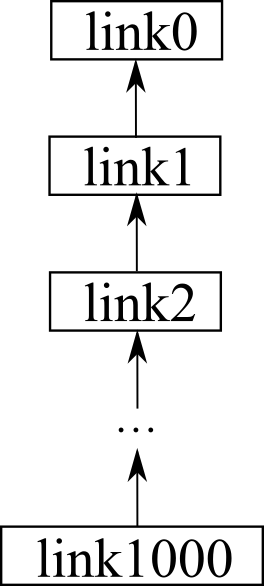
\includegraphics[width=2cm]{snake}	
\caption{ヘビ型ロボットにおける森構造}
\label{fig:snake}
\end{figure}

例えば、ヘビ型ロボットの各関節をTFライブラリで管理する場合について考える。関節の数が1000あり、各関節をフレームとしてTFに登録する場合には図\ref{fig:snake}のよう比較的巨大な森構造になる。森構造の一部のフレーム間の座標変換情報のみ更新するスレッドと、森構想の一部のフレーム間の座標変換情報のみ取得するスレッドがそれぞれ複数あった場合、それぞれのスレッドが森構造の別の部分にアクセスするにもかかわらず、一つのスレッドが森構造にアクセスするたびに森構造全体がロックされてしまいパフォーマンスに多大な影響を及ぼす。

\subsection*{問題2: データの鮮度}
森構造が図\ref{fig:multitree}、タイムラインが図\ref{fig:general-timeline}の状況において、lookupTransformを用いてフレームcからフレームdへの最新の座標変換を計算する時には時刻Aの時点での各フレーム間の座標変換データを用いる。この時、b$\rightarrow$aにおいては最新のデータを用いるが、c$\rightarrow$bにおいては最新のデータと一つ前のデータから線形補間されるデータを用いている。d$\rightarrow$aにおいては最新のデータ$\theta$ではなく一つ前のデータ$\alpha$とそのもう一つ前のデータ$\beta$から線形補間されるデータを用いている。このように、lookupTransformは二つのフレーム間の座標変換の計算において、フレーム間のパスの全てにおいて座標変換データを提供できる時刻についての座標変換を計算するという仕様のため、b$\rightarrow$aのように座標変換情報の登録が遅れるとそれに足を引っ張られてしまい、最新の座標変換データが使われなくなるという問題がある。時刻の同期をとっているためデータの同期性はあるが、最新のデータが使われなくなる可能性があり、データの鮮度は失われる。現在、TFライブラリには最新の座標変換データをもとにフレーム間の座標変換計算をするインターフェイスは無い。

\chapter{提案手法}
本研究では、データベースの並行性制御技術における細粒度ロッキング法及びトランザクション技術における2PLを適用し、これらの問題を解決する。

前述した問題1については、データベースの並行性制御技術における細粒度ロッキング法を適用して解決する。

図\ref{fig:giant-lock}の森構造においてスレッド1がlookupTransformを用いてフレームcからフレームaへの座標変換の計算、スレッド2がsetTransformを用いてフレームdからフレームaへの座標変換を更新する場合について考える。ここで、スレッド1はフレームcとフレームbのデータの読み込み、スレッド2はフレームdのデータの書き込みを行うため、スレッド$i$のデータ$x$に対する読み込み操作を$r_i(x)$、スレッド$i$のデータ$x$に対する書き込み操作を$w_i(x)$と表記すると、スレッド1の操作は$r_1(c)r_1(b)$、スレッド2の操作は$w_2(d)$と表記できる。


\begin{figure}[h] 
\centering
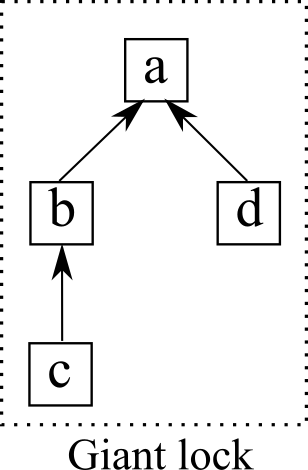
\includegraphics[width=4cm]{gaint-lock}	
\caption{Giant lock}
\label{fig:giant-lock}
\end{figure}


TFライブラリでは森構造へのアクセスをする際、森構造全体をジャイアント・ロックする。これにより、図\ref{fig:giant-lock}の点線枠部分が保護される。図\ref{fig:g-lock-time}はスレッド1の処理中にスレッド2の処理が開始した時のスケジュールを図示している。セルが実行中の処理を表し、セルの端のGlockとGunlockは森構造へのジャイアントロック、アンロックを表す。スレッド2の処理が開始した時、スレッド1が森構造をジャイアントロックしているため、スレッド2はスレッド1の処理が完了し森構造のロックが外されるまで待機する必要がある。スレッド1がアクセスするデータとスレッド2がアクセスするデータは異なるため、より細かくロックする範囲を指定できる方法があればスレッド2がスレッド1の処理の完了を待つ必要がなくなる。


\begin{figure}[h] 
\centering
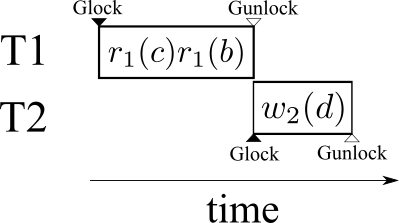
\includegraphics[width=7cm]{g-lock-time.png}	
\caption{ジャイアントロックにおけるスケジュール}
\label{fig:g-lock-time}
\end{figure}

そこで、本研究ではデータベースの並行性制御技術における細粒度ロッキング法を適用する。
細粒度ロッキング法ではアクセスするデータにのみロックをかけ、さらにロックの種類を読み込みロックと書き込みロックに分ける。
複数のスレッドが同じデータにアクセスする際に発生するデータ競合を避けるために、排他制御では一つのスレッドからのみデータにアクセスできるようにするため、ロックをかける。しかしながら、複数のスレッドが同じデータにアクセスする際、データの読み込みのみ行うのであればデータ競合は発生しない。そこで、データの読み込みのみを行う時には読み込みロック、データの書き込みを行う時には書き込みロックを使い、次のようなルールを設ける。

\begin{itemize}
 \item 読み込みを行う前に読み込みロック、書き込みを行う前に書き込みロックを行う必要がある
 \item ロックされていないデータには読み込みロック、及び書き込みロックをかけられる
 \item すでに読み込みロックされたデータにも他のスレッドが読み込みロックをかけることができる
 \item すでに読み込みロックされたデータには他のスレッドが書き込みロックをかけることはできない
 \item すでに書き込みロックされたデータには他のスレッドは読み込みロックも書き込みロックもかけることはできない
\end{itemize}


\begin{table}[h!]
\centering
\begin{tabular}{ | m{1cm} | m{1cm} | m{1cm} | } 
  \hline
  & $rl_i(x)$ & $wl_i(x)$ \\ 
  \hline
  $rl_j(x)$ & $\circ$ & $\times$ \\ 
  \hline
  $wl_j(x)$ &  $\times$ & $\times$ \\ 
  \hline
\end{tabular}	
\caption{lock table}
\label{table:各ロックの互換性}
\end{table}


このルールは、表\ref{table:lock-table}のような表形式で説明することもできる。表中ではスレッド$i$のデータ$x$に対する読み込みロック操作を$rl_i(x)$、スレッド$i$のデータ$x$に対する書き込みロック操作を$wl_i(x)$と表記する。表は一行目がスレッド$i$によってロックがかけられている状態を表し、その状態に読み込みロック、または書き込みロックをスレッド$j(i \neq j)$がかけられるかどうかを2、3行目で表している。$\circ$はすでにロックがかかっていても別のスレッドがロックをかけられることを表し、$\times$はそうでないことを表す。例えば、2行2列目はすでに$rl_i(x)$がかかっていても$rl_j(x)$がかけられることを表し、2行3列目はすでに$wl_i(x)$がかかっていると$rl_j(x)$はかけられないことを表す。

\begin{figure}[h] 
\centering
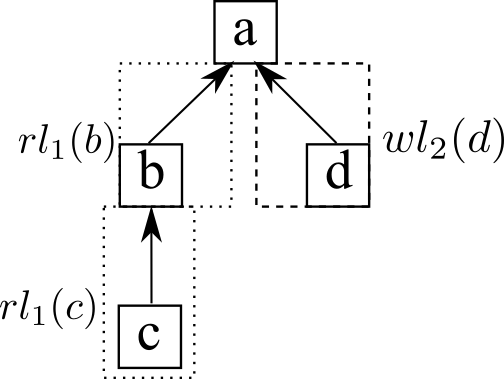
\includegraphics[width=7cm]{high-gran-lock}
\caption{細粒度ロッキング}
\label{fig:high-gran-lock}
\end{figure}


\begin{figure}[h] 
\centering
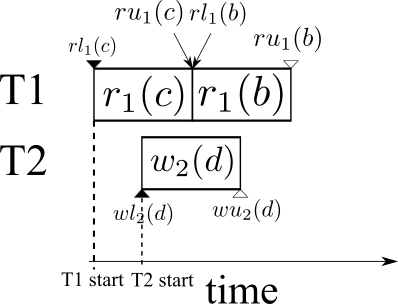
\includegraphics[width=7cm]{high-gran-time}
\caption{細粒度ロックにおけるスケジュール}
\label{fig:high-gran-time}
\end{figure}



細粒度ロッキングを用いた場合のスレッド1、スレッド2の保護範囲は図\ref{fig:high-gran-lock}、スケジュールは図\ref{fig:high-gran-time}で表せる。図\ref{fig:high-gran-time}ではスレッド$i$がデータ$x$を読み込みアンロック、書き込みアンロックする時にはそれぞれ$ru_i(x), wu_i(x)$と表記される。

スレッド1の実行中にスレッド2の処理が開始しても、図\ref{fig:high-gran-lock}で表されるようにスレッド1とスレッド2でアクセスするデータは異なるため、スレッド2はスレッド1の処理完了を待機する必要がなくなる。このスケジュールは各操作を時系列順に表記することにより$rl_1(c)r_1(c)wl_2(d)w_2(d)ru_1(c)rl_1(b)r_1(b)wu_2(d)ru_1(b)$と書ける。


\begin{figure}[h] 
\centering
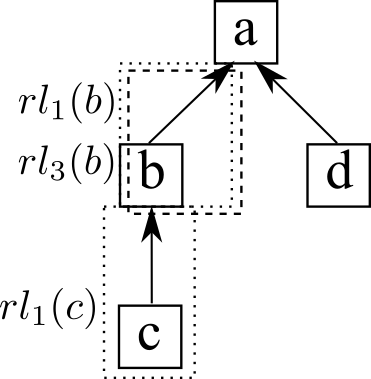
\includegraphics[width=5cm]{two-read-lock}
\caption{二つの読み込みロック}
\label{fig:two-read-lock}
\end{figure}


\begin{figure}[h] 
\centering
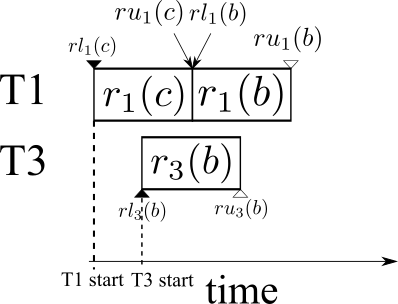
\includegraphics[width=7cm]{two-read-lock-time}
\caption{二つの読み込みロックにおけるスケジュール}
\label{fig:two-read-lock-time}
\end{figure}

スレッド1の処理の途中に、lookupTransformを用いてフレームdのデータを読み込むスレッド3が開始するケースについて考える。細粒度ロッキングを用いた場合のスレッド1とスレッド3の保護範囲は図\ref{fig:two-read-lock}で、スケジュールは図\ref{fig:two-read-lock-time}で表記される。スレッド1にてデータbに対して読み込みロックを取るときすでにスレッド3がbを読み込みロックしているが、表\ref{table:lock-table}が表すようにすでに読み込みロックがかけられていても他のスレッドが読み込みロックをかけることができる。このスケジュールは$rl_1(c)r_1(c)rl_3(b)r_3(b)ru_1(c)rl_1(b)r_1(b)ru_3(b)ru_1(b)$と書ける。


このように、細粒度ロッキング法ではデータごとにロックをし、さらに読み込みロック・書き込みロックと区別をつけることにより並行性を上げることができる。

、細粒度ロックを実装したlookupTransform、getLatestCommonTimeの擬似アルゴリズムをそれぞれアルゴリズム\ref{algo:lookupTransform2}、アルゴリズム\ref{algo:getLatestCommonTime2}にて示す。

\begin{algorithm}
  \caption{細粒度ロックを実装したlookupTransform}\label{algo:lookupTransform2}
\begin{algorithmic}[1]
	\Function {lookupTransform}{target, source, time} 
	\If{time == 0}
	\State{time = getLatestCommonTime(target, source)}
	\EndIf
	\State source\_trans = $I$
	\State frame = source
	\State top\_parent = frame
	\While{frame $\neq$ root}
	\State frame.rLock()
	\State (trans, parent) = frame.getLatestTransAndParent() 
	\State frame.rUnlock()
	\State source\_trans *= trans
	\State top\_parent = frame
	\State frame = parent
	\EndWhile
	\State frame = target
	\State target\_trans = $I$
	\While{frame $\neq$ top\_parent}
	\State frame.rLock()
	\State (tarns, parent) = frame.getTransAndParent(time)
	\State frame.rUnlock()
	\State target\_trans *= trans
	\State frame = parent
	\EndWhile
	
	\Return source\_trans * (target\_trans)$^{-1}$
	\EndFunction
\end{algorithmic}
\end{algorithm}

\begin{algorithm}
\caption{細粒度ロックを実装したgetLatestCommonTime} \label{algo:getLatestCommonTime2}
\begin{algorithmic}[1]
	\Function{getLatestCommonTime}{target, source} 
	\State frame = source
	\State common\_time = TIME\_MAX
	\State lct\_cache = [ ] 
	\While{frame $\neq$ root}
	\State frame.rLock()
	\State (time, parent) = frame.getLatestTimeAndParent()
	\State frame.rUnLock()
	\State common\_time = min(time, common\_time)
	\State lct\_cache.push\_back((time, parent))
	\State frame = parent
	\EndWhile
	\State frame = target
	\State common\_time = TIME\_MAX
	\While{true}
	\State frame.rLock()
	\State (time, parent) = frame.getLatestTimeAndParent()
	\State frame.rUnLock()
	\State common\_time = min(time, common\_time)
	\If{parent \textbf{in}  lct\_cache}
	\State common\_parent = parent
	\State \textbf{break}
	\EndIf
	\State frame = parent
	\EndWhile
	\For{(time, parent) \textbf{in} lct\_cache}
	\State common\_time = min(common\_time, time)
	\If{parent == common\_parent}
	\State \textbf{break}
	\EndIf
	\EndFor
	\Return common\_time
	\EndFunction
\end{algorithmic}
\end{algorithm}


前述した問題2については、複数の座標変換のデータをatomicに取得するインターフェース(lookupLatestTransform)、及び複数の座標変換の最新のデータをatomicに更新するインターフェース(setTransforms)を提供して解決する。setTransformsインターフェイスの必要性について説明する。

まず、二つのフレーム間の座標変換を計算する際に線形補間を行わずにフレーム間のパスの最新の座標変換データを使うインターフェイスとしてlookupLatestTransformを導入する。これは森構造が図\ref{fig:multitree}、タイムラインが図\ref{fig:general-timeline}における状況でフレームcからフレームdへの座標変換は次のように計算される。

\begin{enumerate}
	\item フレームcから木構造のルートノードへパスをたどりながら、各フレーム間の最新の座標変換を掛け合わせてフレームから木構造のルートノードへの座標変換を計算する。ここでは、フレームcから木構造のルートノードへのパスはc$\rightarrow$b、b$\rightarrow$aとなり、それぞれの座標変換は最新のものを使う。
	\item 同じように、フレームdから木構造のルートノードへパスをたどりながら、各フレーム間の最新の座標変換を掛け合わせてフレームから木構造のルートノードへの座標変換を計算する。
	\item フレームcから木構造のルートノードへの座標変換と、木構造のルートノードからフレームdへの座標変換を掛け合わせる。木構造のルートノードからフレームdへの座標変換はフレームdから木構造のルートノードへの座標変換の逆変換から得られる。
\end{enumerate}

\begin{figure}[h] 
\centering
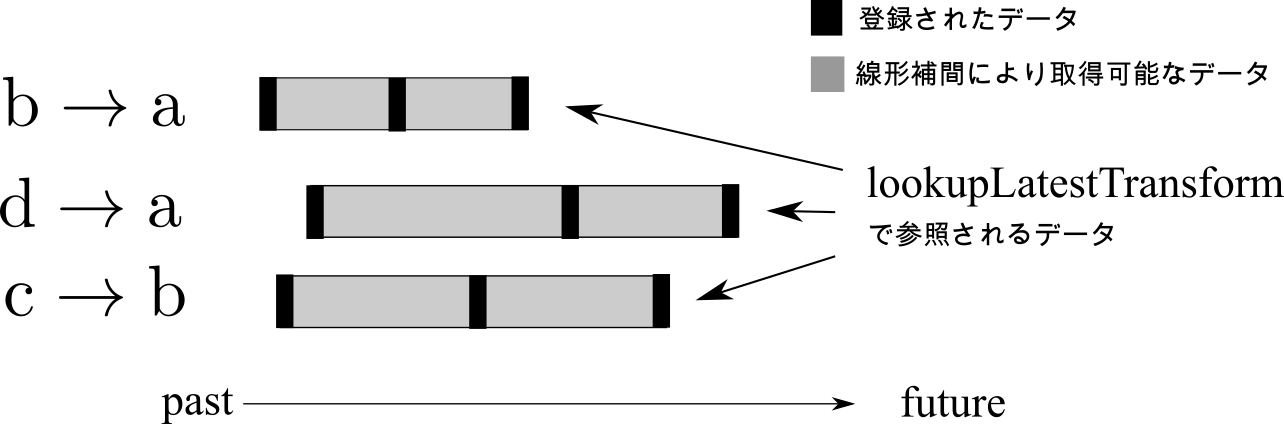
\includegraphics[width=12cm]{lookupLatestTransform}
\caption{lookupLatestTransformで取得するデータ}
\label{fig:lookupLatestTransform}
\end{figure}

lookupLatestTransformにて取得する座標変換データは、図\ref{fig:lookupLatestTransform}のように図示できる。

lookupLatestTransformを新たに提供することにより、暗黙的な線形補間をさけ、最新の座標変換データをもとにしたフレーム間の座標変換が計算できる。しかし、これには次のようなケースでは問題となる。

\begin{figure}[h] 
\centering
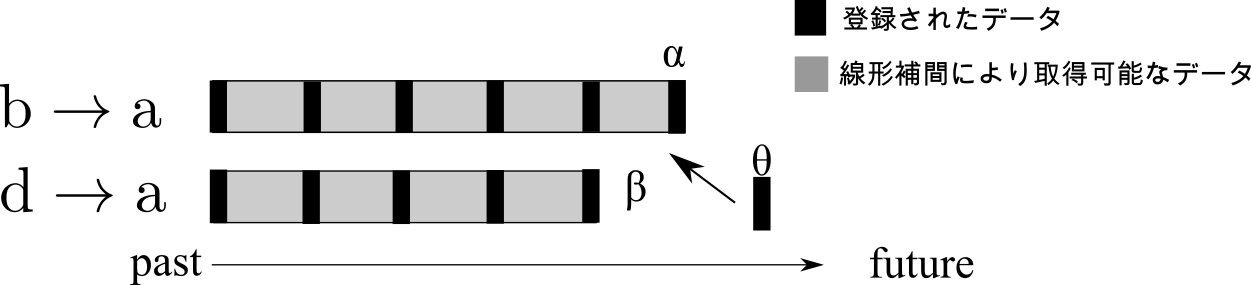
\includegraphics[width=12cm]{coming-same-time}
\caption{同時に座標変換が登録されるケース}
\label{fig:coming-same-time}
\end{figure}


図\ref{fig:coming-same-time}は森構造が図\ref{fig:multitree}の時にフレームbからフレームaへの座標変換と、フレームdからフレームaへの座標変換が同時刻に登録されるケースでのタイムラインを表す。
b$\rightarrow$aとa$\rightarrow$cのデータを用いてフレームbからフレームcへの座標変換を計算する際、ユーザーはb$\rightarrow$aとd$\rightarrow$aのデータについては同時刻のものを使うことを期待する。しかしながら、lookupLatestTransformを使うとユーザーの期待に反して図\ref{fig:coming-same-time}のように$\theta$がまだ登録されていない中間状態のタイムラインを観測し、$\alpha$と$\beta$を元に座標変換してしまうことがある。これは、複数の座標変換の登録においてsetTransformを複数呼び出す際、 全ての座標変換が登録できていない状態でlookupLatestTransformが森構造にアクセスできることに起因する。従来のlookupTransformではフレーム間のパスの全てにおいて座標変換データを提供できる時刻についての座標変換を計算するという仕様のため、このような問題は発生しなかった。

% ただの細粒度ロックだとSerializabilityがなくなる、けどgiant lockだとパフォーマンスがまずいという話を説明する必要はある?

そこで、複数の座標変換を2PLによってatomicに森構造に登録するsetTransformsを提供し、またlookupLatestTransformも2PLを使うように変更する。2PL\cite{2PL}とは、複数のデータに対するロック・アンロックを二つのフェーズに分けることによって並行処理の結果が直列処理と同じ結果になることを保証する、データベースにおけるトランザクション技術である。このような性質は、Serializabilityと呼ばれる。

%TODO Serializabilityはどこから引用?

2PLによって並行性制御をしたときのsetTransformsとlookupLatestTransformの動作について説明する。スレッド1がsetTransformsを用いてb$\rightarrow$a、d$\rightarrow$aの情報を更新し、スレッド2がlookupLatestTransformを用いてb$\rightarrow$a、d$\rightarrow$aの情報を元にフレームbからフレームdへの座標変換を計算し、スレッド1の処理中にスレッド2の処理が開始するケースについて考える。それぞれのスレッドの処理は$w_1(b)w_1(d)$、$r_2(b)r_2(d)$と表現できる。

\begin{figure}[h] 
\centering
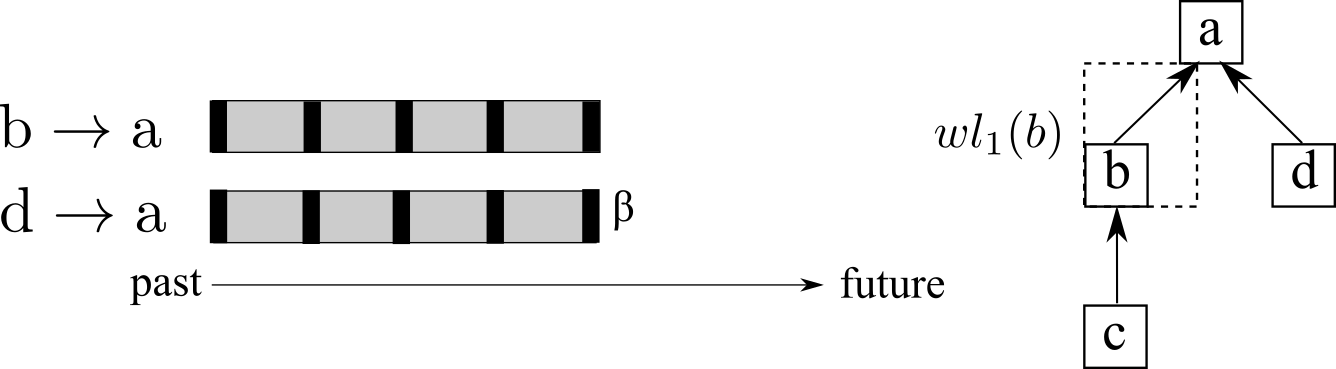
\includegraphics[width=12cm]{setTransforms1}
\caption{setTransformsとlookupLatestTransform 1}
\label{fig:setTransforms1}
\end{figure}

図\ref{fig:setTransforms1}はスレッド1で$w_1(b)$をする前に$wl_1(b)$をした時の様子を表している。この状態でスレッド2の処理が始まると、$r_2(b)$をするために$rl_2(b)$を確保する必要があるが、まだ$wl_1(b)$がかけられているためにロックが外されるまで待つ必要がある。

\begin{figure}[h] 
\centering
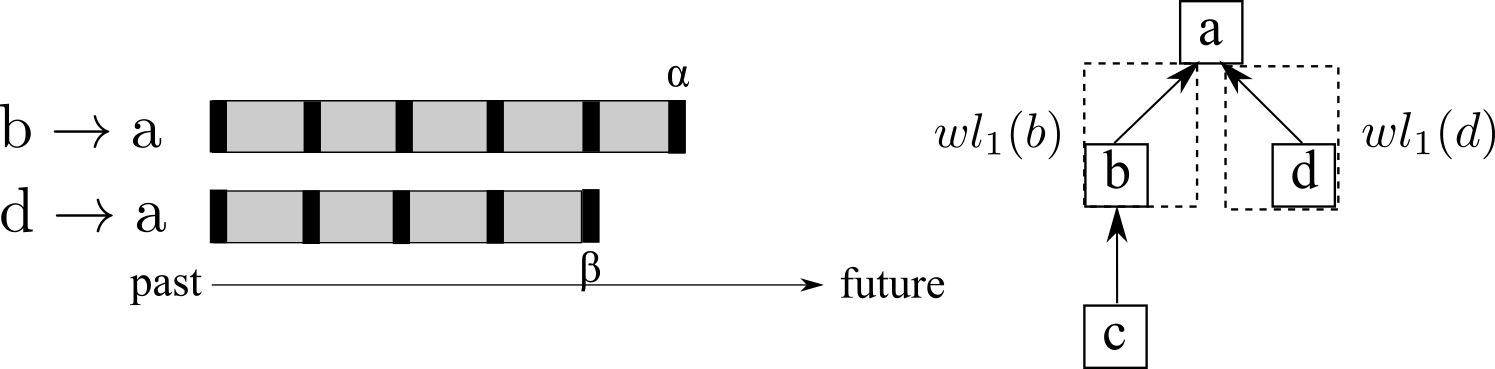
\includegraphics[width=12cm]{setTransforms2}
\caption{setTransformsとlookupLatestTransform 2}
\label{fig:setTransforms2}
\end{figure}

図\ref{fig:setTransforms2}はスレッド1で$w_1(b)$が完了してデータ$\alpha$が登録され、$w_1(d)$をする前に$wl_1(d)$をした時の様子を表している。2PLでは複数のロックを確保し、必ず全てのロックを取り終えてからアンロックをしていく。このため、bへのロックはまだ解放されておらずスレッド2は待機する必要がある。


\begin{figure}[h] 
\centering
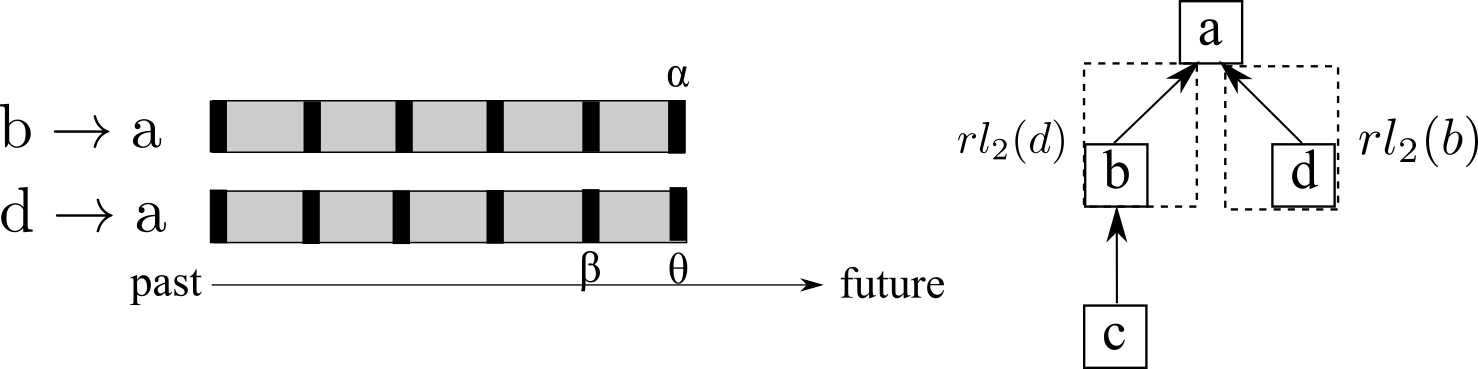
\includegraphics[width=12cm]{setTransforms3}
\caption{setTransformsとlookupLatestTransform 3}
\label{fig:setTransforms3}
\end{figure}


図\ref{fig:setTransforms3}はスレッド1の処理が完了してデータ$\theta$が登録され、スレッド1によるフレームb,dへのロックが開放され、スレッド2が$r_2(b)$と$r_2(d)$をするために$rl_2(b)$と$rl_2(d)$のロックを確保した時の様子である。2PLによりスレッド1の処理が完了してからスレッド2は森構造へアクセスできるため、スレッド2が中間の状態を観測することはなくなる。

この一連のスケジュールは$wl_1(b)w_1(b)wl_1(d)w_1(d)wu_1(b)wu_1(d)rl_2(b)r_2(b)rl_2(d)r_2(d)ru_2(b)ru_2(d)$と表記できる。

さて、2PLによって複数のデータに対する読み込み・書き込みがatomicに行えるようになったが、複数のデータに対してロックを取ることによりdeadlockの可能性が生じる。


\begin{figure}[h] 
\centering
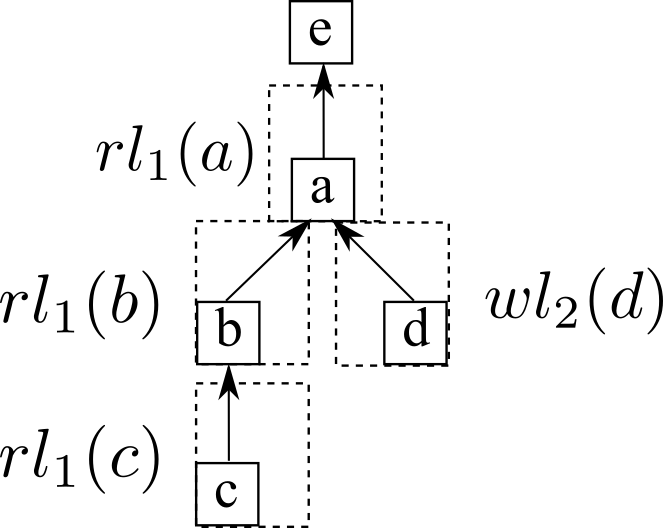
\includegraphics[width=5cm]{deadlock}
\caption{deadlock}
\label{fig:deadlock}
\end{figure}

図\ref{fig:deadlock}のような森構造において、スレッド1がフレームcからフレームdへの座標変換をlookupLatestTransformを用いて計算し、スレッド2がsetTransformsを用いてd$\rightarrow$a及びa$\rightarrow$eの座標変換を更新する場合について考える。それぞれのスレッドの操作は$r_1(c)r_1(b)r_1(a)r_1(d)$、$w_2(d)w_2(a)$と表記できる。

図\ref{fig:deadlock}はスレッド1がa, b, cの読み込みロック、スレッド2がdの書き込みロックを確保した状態を表している。ここで、スレッド1は次にdの読み込みロックを確保したいがすでにスレッド2がdを書き込みロックしているためロックの解放を待機する必要がある。スレッド2は次にaの書き込みロックを確保したいがすでにスレッド1がaを読み込みロックしているために待機する必要がある。二つのスレッドがお互いのロック解放を待ち続けるため、deadlockとなる。これはスレッド2が森構造のルートノードへ登る方向にロックをかけているのに対し、スレッド1は逆に一時的に森構造を下る方向にロックをかけていることに起因する。

% 要素のreorderによって防げるけどちょいとむずそう

そこで、我々はdeadlockを未然に防ぐ方法としてNoWait\cite{nowait}を採用した。これは、書き込みロックを2つ以上かけようとしたときにすでにデータがロックされていたら、保持しているロックを全て解放し最初から処理をやり直す手法である。これにより、書き込みロックを2つ以上しているスレッドがロックの解放を待機することがなくなり、deadlockは発生しない。また、我々の手法ではcontention regulationとして保持しているロックを全て解放して1ミリ秒経過してから最初から処理をやり直す。

\begin{figure}[h] 
\centering
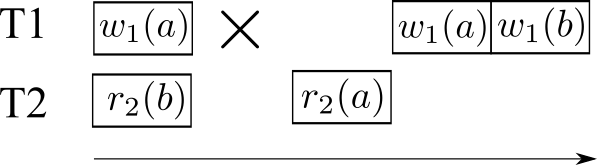
\includegraphics[width=10cm]{dirty-read}
\caption{Dirty Read}
\label{fig:dirty-read}
\end{figure}


NoWaitによって処理のやり直しが発生するため、setTransformsでは書き込みを行うタイミングに注意する必要がある。T1がsetTransformsを用いて$w_1(a)w_1(b)$、T2がlookupLatestTransformを用いて$r_2(b)r_2(a)$を実行する時、図\ref{fig:dirty-read}のようなスケジュールになったケースについて考える。T1が$a$の書き込みを終えた後に$b$への書き込みロックを取ろうとするが、すでにT2によって$b$への読み込みロックは取られているので、NoWaitによって$a$へのロックを外してから処理をやり直す。T1による処理のやり直しの前にT2が$a$を読み込んでしまうと、T2は$a$についてはT1による更新後のデータ、$b$についてはT1による更新前のデータを読んでしまい、並行処理の結果が直列処理と同じ結果にならなくなってしまう。この問題は、トランザクション理論においてはDirty readと呼ばれる。

Dirty readを避けるため、我々の手法では全ての書き込みロックが確保できてから座標変換の書き込みを行うようにした。これにより、書き込みが一部行われた状態を読み込み専用スレッドが観測することはなくなる。

\begin{figure}[h] 
\centering
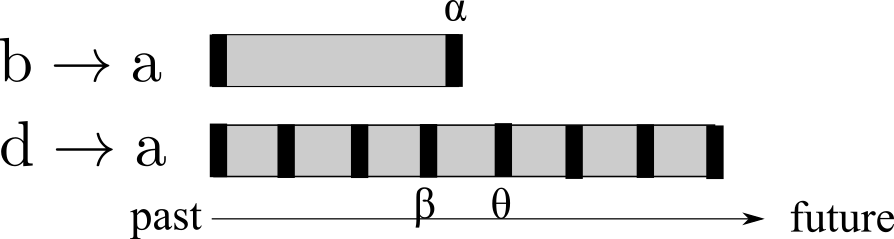
\includegraphics[width=10cm]{need-many-update}
\caption{deadlock}
\label{fig:need-many-update}
\end{figure}


setTransformsとlookupLatestTransformを利用すると、最新の座標変換を更新・取得できるだけではなく、無駄な座標変換の更新も減らすことができる。図\ref{fig:need-many-update}において、b$\rightarrow$aはあまり座標系間の位置関係が変わらないために座標変換はあまり更新されないが、d$\rightarrow$aの座標変換は頻繁に更新されるケースについて考える。座標変換の計算においてb$\rightarrow$aとd$\rightarrow$aのデータを用いる場合、既存のTFでは「該当する時刻の座標変換データが保存されている、もしくは前後の値を元に線形補間ができる場合にはその時刻の座標変換データを提供できると見做す」という仕様により、b$\rightarrow$aの更新が遅いためにd$\rightarrow$aでは過去の鮮度の低い$\beta$と$\theta$から座標変換の計算をしなくてはならない。これを避けるため、既存のTFではあまり座標系間の位置関係が変わらないb$\rightarrow$aにおいても、一定周期で同じ座標変換情報を登録する必要があった。このように、既存のTFでは座標変換情報が変わらないにもかかわらず一定周期で同じ座標変換情報を登録する必要があり、余計な負荷がかかっていた。しかしながら、setTransformsと
lookupLatestTransformでは最新の座標変換のみを見るため必要な時にのみ座標変換の更新をすればよく、このような余計な負荷がかかることは無くなる。

% でも、TFは同期を取ったほうがいいとされるからああいう設計にしたんじゃ?最新のデータだけ保存するようにしてればよかったじゃん
%TODO ここ突っ込まれたら痛いなああああ、ここの回答は「この研究を通して既存のTFもそうなってくれると嬉しいですね」程度のコメントで

lookupLatestTransform、setTransformsの擬似アルゴリズムをそれぞれアルゴリズム\ref{algo:lookupLatestTransform}、\ref{algo:setTransforms}にて示す。

\begin{algorithm}
  \caption{lookupLatestTransform}\label{algo:lookupLatestTransform}
\begin{algorithmic}[1]
	\Function {lookupLatestTransform}{target, source}
	\State rlock\_list = [ ]
	\State source\_trans = $I$
	\State frame = source
	\State top\_parent = frame
	\While{frame $\neq$ root}
	\State rlock\_list.push\_back(frame)
	\State (trans, parent) = frame.getLatestTransAndParent() 
	\State source\_trans *= trans
	\State top\_parent = frame
	\State frame = parent
	\EndWhile
	\State frame = target
	\State target\_trans = $I$
	\While{frame $\neq$ top\_parent}
	\State rlock\_list.push\_back(frame)
	\State (tarns, parent) = frame.getTransAndParent(time)
	\State target\_trans *= trans
	\State frame = parent
	\EndWhile
	\State unlock all in rlock\_list
	
	\Return source\_trans * (target\_trans)$^{-1}$
	\EndFunction
\end{algorithmic}
\end{algorithm}


\begin{algorithm}
\caption{setTransforms}\label{algo:setTransforms}
\begin{algorithmic}[1]
	\Function{setTransforms}{transforms}
	\State wlock\_list = [ ] \label{op1}
	\For{trans in transforms}
	\State frame = getFrame(trans.child\_frame\_id)
	\State lock\_success = frame.tryWLock()
	\If{lock\_success}
	\State wlock\_list.push\_back(frame)
	\Else
	\State unlock all in wlock\_list
	\State sleep 1ms 
	\State \textbf{goto} \ref{op1}
	\EndIf
	\EndFor
	\For{trans in transforms} \Comment{Dirty readを避けるため、全てのwlockが確保できてから書き込み}
	\State frame = getFrame(trans.child\_frame\_id)
	\State frame.insertData(trans)
	\EndFor
	\State unlock all in wlock\_list
	\EndFunction
\end{algorithmic}
\end{algorithm}

\chapter{評価}
TFライブラリに細粒度を実装したlookupTransform・setTransform、及び最新の複数のデータをatomicに取得・更新できるlookupLatestTransform・setTransformsを以下の指標で評価した。

\begin{enumerate}
	\item スループット: 一秒間に何回操作(lookupTransform及びsetTransforms)ができたか
	\item レイテンシ: 操作の応答時間
	\item データの鮮度: lookupTransformにおいてアクセスした各座標変換データのタイムスタンプの新しさを表す。アクセスした各座標変換データのタイムスタンプの平均とアクセス時の時刻の差をdelayとし、delayが少ない方がデータの鮮度が高いとみなす。
	\item データの同期性(lookupLatestTransformのみ): lookupTransformにおいてアクセスした各座標変換データのタイムスタンプの同一性を表す。アクセスした各座標変換データのタイムスタンプの標準偏差を計算し、これが小さい方がデータの同期性があるとみなす。
	\item abort率(setTransformsのみ): setTransformsにおいて、NoWaitによって操作をやり直した回数の比率。(やり直した回数 / setTransformsを呼び出した回数) で求める。
\end{enumerate}

以下、既存手法はold、細粒度ロックを実装したlookupTransform・setTransformsをsnapshot、2PLを用いて複数のデータをatomicに取得・更新できるlookupLatestTransform・setTransformsをlatestと呼称する。



\section{実験環境}

実験にはIntel(R) Xeon(R) Platinum 8176 CPU @ 2.10GHzを4つ搭載したサーバを利用する。それぞれのコアは32KB private L1dキャッシュ、1024KB private L2キャッシュを持つ。単一プロセッサの28コアは39MB L3キャッシュを共有し、ハイパー・スレッディングを有効化している。トータルキャッシュサイズはおよそ160MBである。メモリはDDR4-2666が48個接続されており、一つあたりのサイズは32GB、全体のサイズは1.5 TBである。全ての実験において,実行時間は 60秒という安定的な結果が得られる時間を選択している。

\section{ワークロード}

% Applicationはどこにかく?
実験のワークロードは、関節数が多いヘビ型ロボットの関節情報をTFに登録することを想定し、図\ref{fig:snake}のようなフレーム間の座標変換情報が一直線に与えられた構造に複数のスレッドからアクセスし計測を行う。TFライブラリへのアクセスパターンとしては、主にlookupTransformのみを複数回呼び出すスレッドとsetTransformのみを複数回呼び出すスレッドに二分される。このため、lookupTransformのみを複数回呼び出すスレッド(読み込み専用スレッド)、及びsetTransformのみを複数回呼び出すスレッド(書き込み専用スレッド)をそれぞれ複数立ち上げ計測を行う。

実験においては以下のパラメータが存在する。
\begin{enumerate}
  \item thread: 合計スレッド数
  \item joint: フレームの数
  \item read\_ratio: 合計スレッド数のうち、読み込み専用スレッドの割合
  \item read\_len: 読み込み専用スレッドにて一回のlookupTransform操作で読みこむフレームの数。joint個のフレームのうちランダムにi番目のフレームが選択され、そこからi+read\_len番目のフレームまでの座標変換が計算される。
  \item write\_len: 書き込み専用スレッドにて一回の操作で座標変換情報を更新するフレームの数。joint個のフレームのうちランダムにi番目のフレームが選択され、そこからi+read\_len番目のフレームまでの座標変換が更新される。setTransformでは一度に一個のフレームしか更新できないためwrite\_len回setTransformを呼び出す操作を一つの操作とする。
  \item frequency: 各スレッドにて操作を呼び出す周期。操作の呼び出しが完了したのち、1 / frequency秒待機してから再び操作を呼びだす。0に設定すると待機なしで操作を呼び出し続ける。各スレッドが一定の周期にて操作を呼び出すというのは、ROSにおいて一般的なワークロードである。
  \item opposite\_write: 本実験において、読み込み専用スレッドは図\ref{fig:opposite-write}のように下から上に順に読み込みロックをとる。このフラグをtrueにすると、上から下の方向に書き込みロックをとり、読み込みロックとは逆方向にロックをとる。falseにすると下から上の方向に書き込みロックをとる。
\end{enumerate}

\begin{figure}[h] 
\centering
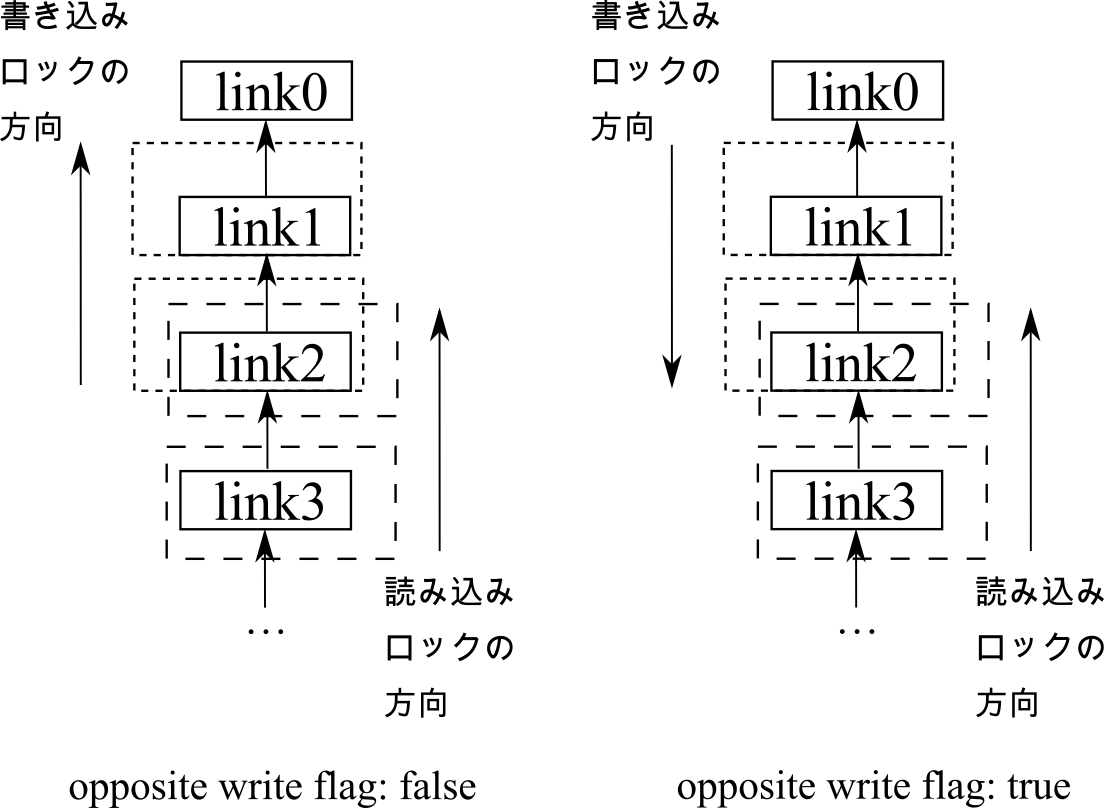
\includegraphics[width=15cm]{opposite-write}
\caption{opposite\_writeフラグ}
\label{fig:opposite-write}
\end{figure}


各実験はそれぞれYCSB-A/B/C\cite{ycsb}ワークロードについて行われている。YCSB-A/B/Cはそれぞれ、読み込み操作と書き込み操作の割合が50:50、95:5、100:0のワークロードを指す。ここでは読み込み専用スレッドの数と書き込み専用スレッドの数の比でそれぞれのワークロードを再現するため、read\_ratioをそれぞれ0.5、0.95、1に設定した。

特に記載がない場合はjoint=10000、read\_len=16、write\_len=16、frequency=0で実験が行われている。
%TODO ここは舛村さんのワークロードを参考にしたが、実際のロボットではreadが全てを読む、writeもたくさん、というケースはあり得そうじゃないか?つまり、一般的なDBのパタンだけじゃだめ。
% あとabortのratioについてもまとめないと

%YCSB-A/B/Cそれぞれで説明した方がわかりやすいかも。C->A->Bとか


\section{YCSB-C}

\begin{figure}[h] 
\centering
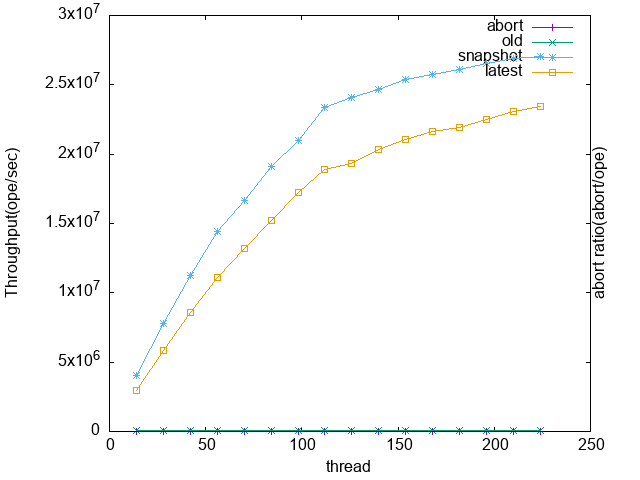
\includegraphics[width=15cm]{data/stable/ycsb-c/throughput}
\caption{YCSB-Cにおけるスレッド数とスループットの関係}
\label{fig:throughput-c}
\end{figure}

\begin{figure}[h] 
\centering
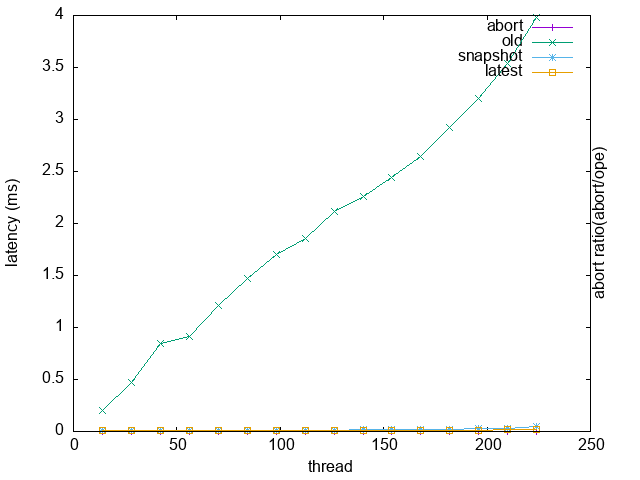
\includegraphics[width=15cm]{data/stable/ycsb-c/latency}
\caption{YCSB-Cにおけるスレッド数とレイテンシの関係}
\label{fig:latency-c}
\end{figure}

\begin{figure}[h] 
\centering
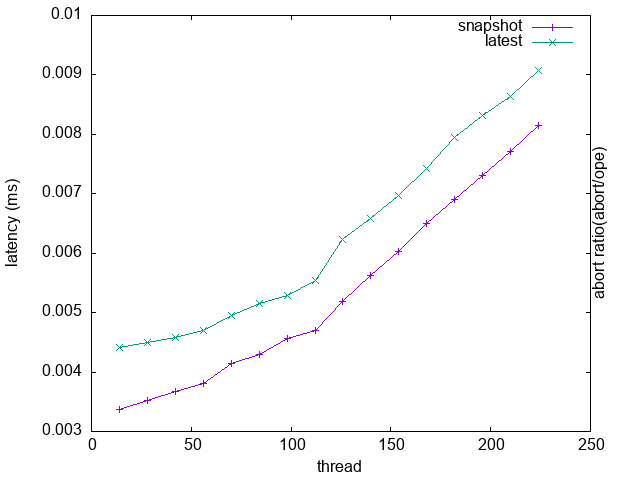
\includegraphics[width=15cm]{data/stable/ycsb-c/latency-2}
\caption{YCSB-Cにおけるスレッド数とレイテンシの関係 snapshotとlatestのみ}
\label{fig:latency-c2}
\end{figure}

スループットについては図\ref{fig:throughput-c}のように、oldに比べてsnapshotは最大455倍、latestは最大393倍のスループットとなった。

レイテンシについては図\ref{fig:latency-c}、図\ref{fig:latency-c2}のように、どの手法においてもレイテンシとスレッド数が線形比例しているが、oldに比べsnapshot、latestは非常に小さいレイテンシとなった。

スループット、レイテンシのどちらにおいてもsnapshotとlatestが優れているのはlatestは2PLによって一度に複数のデータにロックをかけるのに対し、snapshotでは最大一個のデータしかロックしか取らないため、より並行性が高くなると考えられる。

スレッドが112の部分にて、snapshot及びlatestのグラフに傾きが生じているのは、ハイパー・スレッディングによるものだと考えられる。

書き込みが発生しないため、YCSB-Cにおけるデータの鮮度、データの同期性、abort率については説明しない。

\section{YCSB-A}

%TODO 急にスループット下がるのは、キャッシュの取り合い?実際、getLatestCommonのあとで抜けるとこれは改善する

\begin{figure}[h] 
\centering
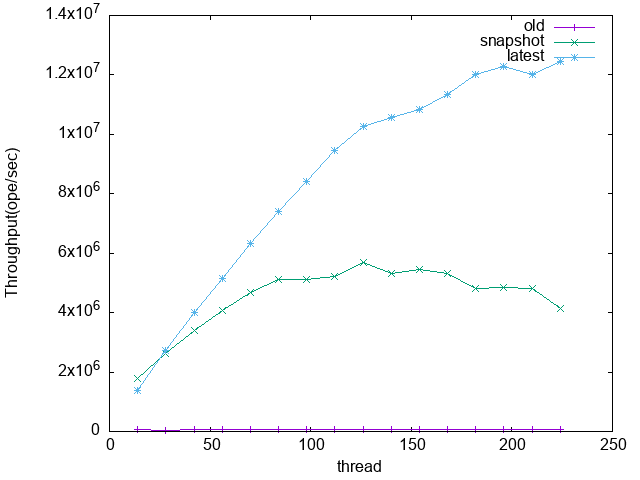
\includegraphics[width=15cm]{data/stable/ycsb-a/news/opposite-throughput}
\caption{opposite\_writeフラグを有効にした場合}
\label{fig:throughput-a-opposite}
\end{figure}

\begin{figure}[h] 
\centering
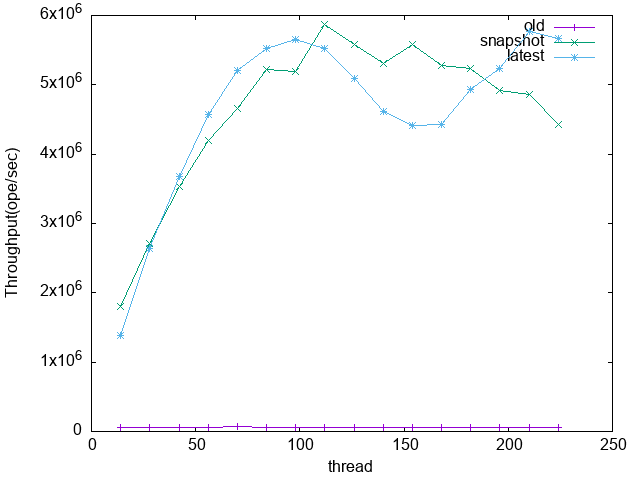
\includegraphics[width=15cm]{data/stable/ycsb-a/news/direct-throughput}
\caption{opposite\_writeフラグを無効にした場合}
\label{fig:throughput-a-direct}
\end{figure}

YCSB-Cとは異なり、YCSB-Aでは書き込み操作が発生するため、opposite\_writeフラグを有効にした場合とそうでない場合に差が生じた。

opposite\_writeフラグを有効にした場合ではスループットについては図\ref{fig:throughput-a-opposite}のようにoldに比べてsnapshotは最大91.3倍、latestは最大203倍のスループットとなり、latestのスループットがsnapshotよりも高くなった。

これに対し、opposite\_writeフラグを無効にした場合ではスループットについては図\ref{fig:throughput-a-direct}のようにoldに比べてsnapshotは最大92倍、latestは最大94倍のスループットとなった。

どちらの場合においてもsnapshotはほとんど変わらないが、latestのスループットには大きな変化が現れた。

\begin{figure}[h] 
\centering
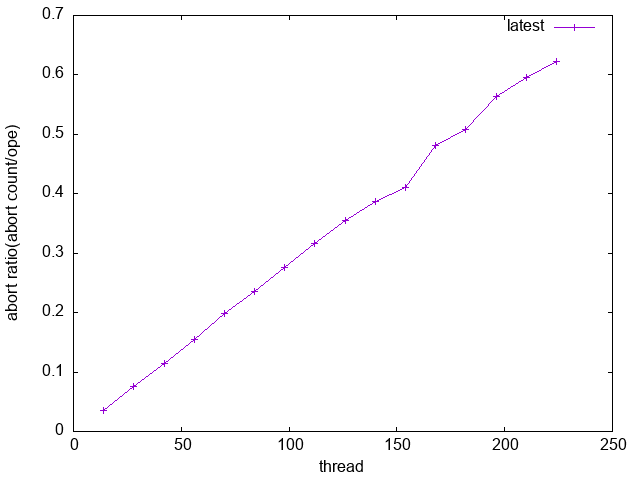
\includegraphics[width=15cm]{data/stable/ycsb-a/news/opposite-abort}
\caption{opposite\_writeフラグを有効にした場合}
\label{fig:a-opposite-abort}
\end{figure}

\begin{figure}[h] 
\centering
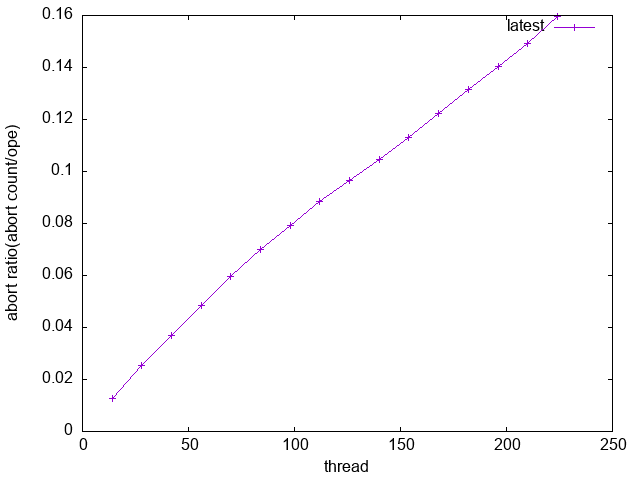
\includegraphics[width=15cm]{data/stable/ycsb-a/news/direct-abort}
\caption{opposite\_writeを無効にした場合}
\label{fig:a-direct-abort}
\end{figure}

なぜこのようになったかを調べるために、まずはabort率について図\ref{fig:a-opposite-abort}、\ref{fig:a-direct-abort}に表示した。どちらもスレッド数に比例してabort率が上がっているが、opposite\_writeが有効になっている方が全体的にabort率が高く、書き込みロックを読み込みロックの逆方向に確保していくとabortしやすいことがわかる。

% ここもっと詳しく?
これは、読み込みロックと同じ方向に書き込みロックをかけた場合には、一番最初の要素に書き込みロックができればその上の要素にabortなしで書き込みロックを取れる可能性が高いのに対し、逆方向に書き込みロックをかけた場合にはいくつかの要素の書き込みロックが取れていても、他の読み込み専用スレッドと衝突し、全ての書き込みロックを外す必要があるため、このようなabort率の差が生じたと考えられる。これにより、読み込みロックと同じ方向に書き込みロックをかけた場合には読み込み専用スレッドは書き込み専用スレッドの完了を待機する必要があるが、逆方向に書き込みロックをかけた場合には書き込み専用スレッドがabortするために待機の必要はなくなると考えられる。


\begin{figure}[h] 
\centering
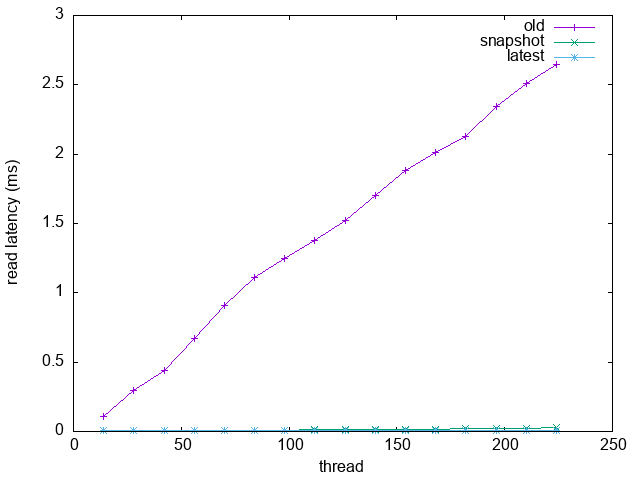
\includegraphics[width=15cm]{data/stable/ycsb-a/news/opposite-read-latency}
\caption{opposite\_writeフラグを有効にした場合}
\label{fig:a-opposite-latency-read}
\end{figure}

\begin{figure}[h] 
\centering
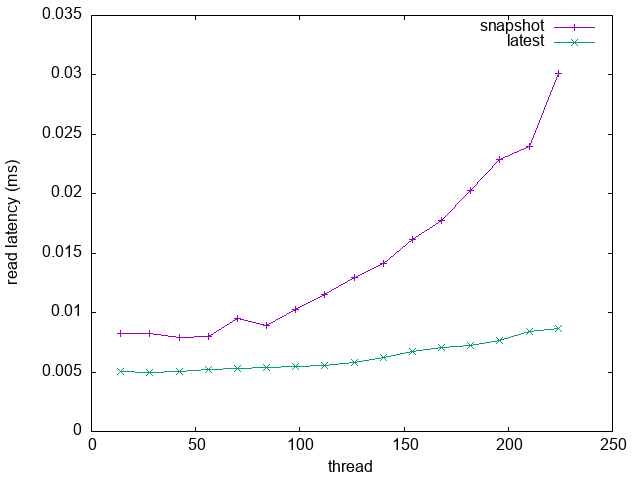
\includegraphics[width=15cm]{data/stable/ycsb-a/news/opposite-read-latency2}
\caption{opposite\_writeフラグを有効にした場合 snapshotとlatestのみ}
\label{fig:a-opposite-latency-read2}
\end{figure}

\begin{figure}[h] 
\centering
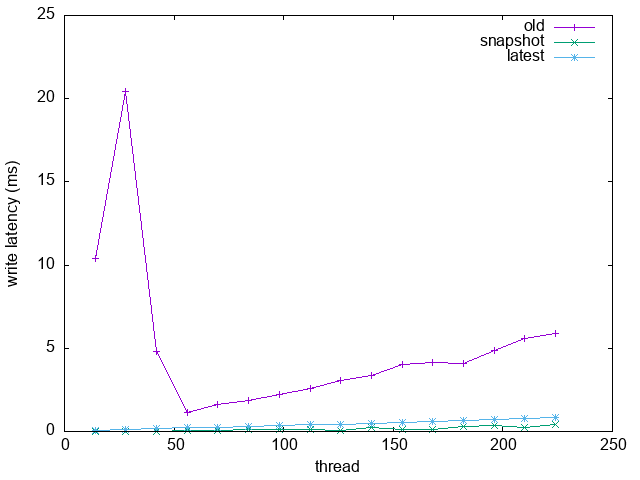
\includegraphics[width=15cm]{data/stable/ycsb-a/news/opposite-write-latency}
\caption{opposite\_writeフラグを有効にした場合}
\label{fig:a-opposite-latency-write}
\end{figure}

\begin{figure}[h] 
\centering
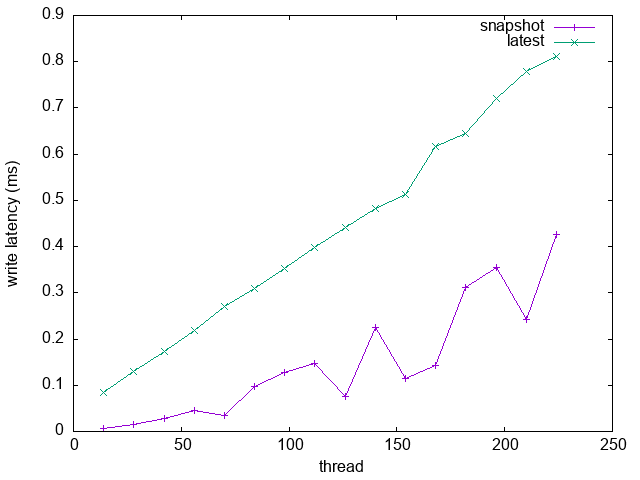
\includegraphics[width=15cm]{data/stable/ycsb-a/news/opposite-write-latency2}
\caption{opposite\_writeフラグを有効にした場合 snapshotとlatestのみ}
\label{fig:a-opposite-latency-write2}
\end{figure}

\begin{figure}[h] 
\centering
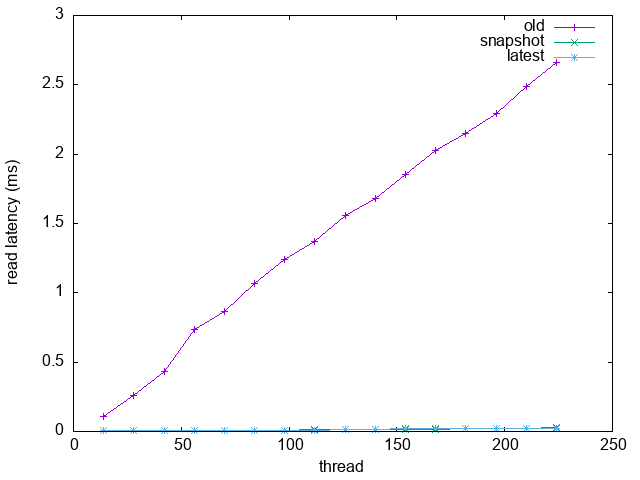
\includegraphics[width=15cm]{data/stable/ycsb-a/news/direct-read-latency}
\caption{opposite\_writeフラグを無効にした場合}
\label{fig:a-direct-latency-read}
\end{figure}

\begin{figure}[h] 
\centering
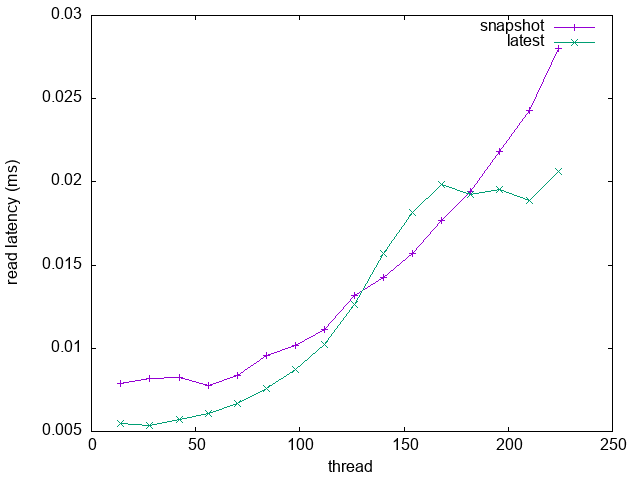
\includegraphics[width=15cm]{data/stable/ycsb-a/news/direct-read-latency2}
\caption{opposite\_writeフラグを無効にした場合 snapshotとlatestのみ}
\label{fig:a-direct-latency-read2}
\end{figure}

\begin{figure}[h] 
\centering
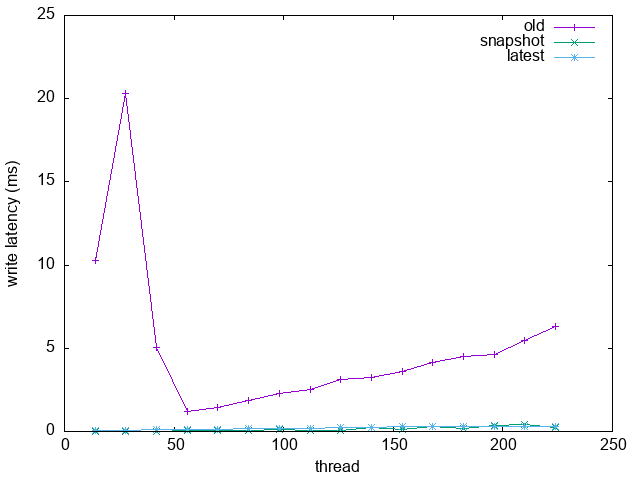
\includegraphics[width=15cm]{data/stable/ycsb-a/news/direct-write-latency}
\caption{opposite\_writeフラグを無効にした場合}
\label{fig:a-direct-latency-write}
\end{figure}

\begin{figure}[h] 
\centering
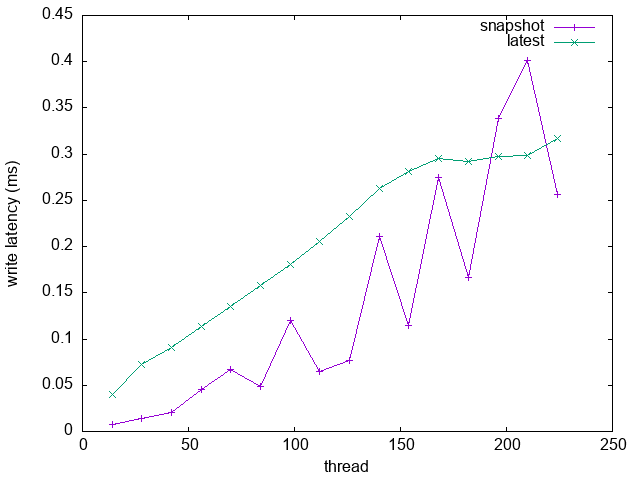
\includegraphics[width=15cm]{data/stable/ycsb-a/news/direct-write-latency2}
\caption{opposite\_writeフラグを無効にした場合 snapshotとlatestのみ}
\label{fig:a-direct-latency-write2}
\end{figure}

次に、読み込み・書き込み専用スレッドそれぞれのレイテンシについて図\ref{fig:a-opposite-latency-read}〜\ref{fig:a-direct-latency-write2}に表示した。

% ここもっと上手くまとめたら?
% グラフを一つにまとめよう!でも厳密にはsetTransformを使っても書き込み順番は変わるし…
% 説明が冗長。

opposite\_writeフラグの有効・無効、読み込み・書き込みに関わらず、どのケースにおいてもsnapshot、latestの方がレイテンシが低いことがわかる。また、opposite\_writeフラグの有効・無効に関わらず、大きな変化がないことがわかる。

図\ref{fig:a-opposite-latency-read2}のように、opposite\_writeフラグが有効な時に読み込みスレッドのレイテンシがlatestがsnapshotより早いのは、snapshotのlookupTransformにおいて二つのフレーム間のパス上の全てのフレームにおいて座標変換を取得できる時刻を検索してから座標変換を計算するために、森構造を2度読み込む必要があるからだと考えられる。

図\ref{fig:a-opposite-latency-write2}のように、opposite\_writeフラグが有効な時に書き込みスレッドのレイテンシがsnapshotがlatestより早いのは、latestのsetTransformsでは一度に複数の要素のロック、書き込みを行い、またNoWaitによってabortし処理をやり直す可能性があるからだと考えられる。

図\ref{fig:a-direct-latency-read2}のように、opposite\_writeフラグが無効な時に読み込みスレッドのレイテンシがlatestがsnapshotとあまり変わらないのは、latestにて書き込みスレッドによるabortが減り、代わりに読み込みスレッドの待機時間が増えたからだと考えられる。これはopposite\_writeフラグが有効な時とは対照的である。

図\ref{fig:a-direct-latency-write2}のように、opposite\_writeフラグが無効な時に書き込みスレッドのレイテンシがlatestがsnapshotとあまり変わらないのは、latestのabortが減ったからだと考えられる。これもopposite\_writeフラグが有効な時とは対照的である。

latestの読み込みスレッドのレイテンシはopposite\_writeフラグが有効な時には最大0.007ms程度、opposite\_writeフラグが無効な時には最大0.02ms程度となる。これに対し、書き込みスレッドのレイテンシはopposite\_writeフラグが有効な時には最大0.8ms程度、opposite\_writeフラグが無効な時には最大0.3ms程度となる。

書き込みのレイテンシと読み込みのレイテンシの倍率はopposite\_writeフラグが有効な時には約100倍、無効な時には約10倍となり、書き込みの方が読み込みよりも時間がかかることがわかる。また、opposite\_writeフラグを有効にすると読み込みのレイテンシは減るが書き込みのレイテンシが増えることがわかる。このことから、opposite\_writeフラグの有効・無効化の選択は読み込みのレイテンシを下げるか、それとも書き込みのレイテンシを下げるかのトレードオフとなると考えられる。

\begin{figure}[h] 
\centering
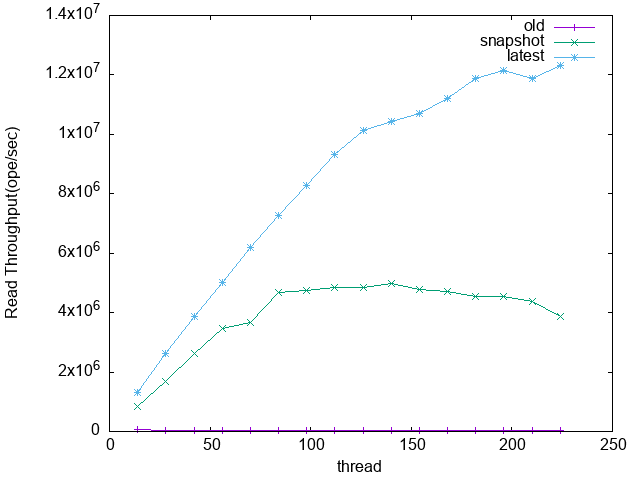
\includegraphics[width=15cm]{data/stable/ycsb-a/news/opposite-read-throughput}
\caption{opposite\_writeフラグを有効にした場合}
\label{fig:a-opposite-throughput-read}
\end{figure}

\begin{figure}[h] 
\centering
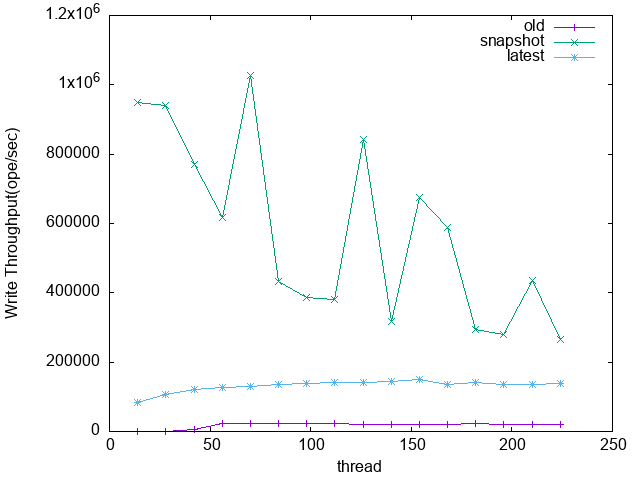
\includegraphics[width=15cm]{data/stable/ycsb-a/news/opposite-write-throughput}
\caption{opposite\_writeフラグを有効にした場合}
\label{fig:a-opposite-throughput-write}
\end{figure}

\begin{figure}[h] 
\centering
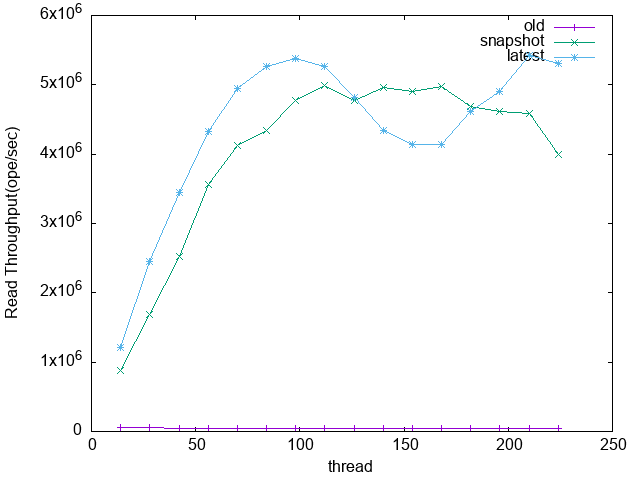
\includegraphics[width=15cm]{data/stable/ycsb-a/news/direct-read-throughput}
\caption{opposite\_writeフラグを無効にした場合}
\label{fig:a-direct-throughput-read}
\end{figure}

\begin{figure}[h] 
\centering
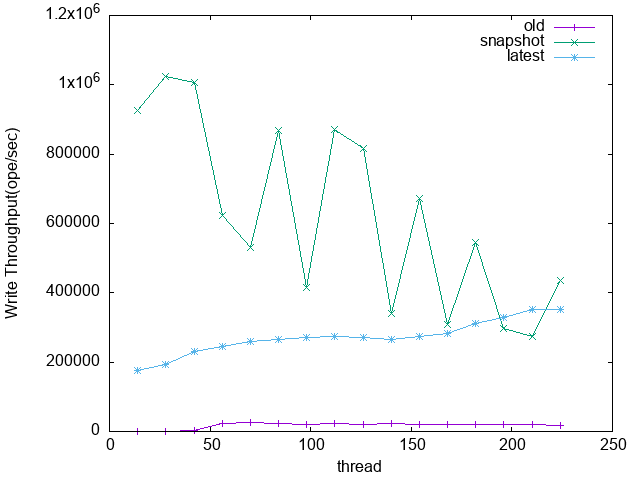
\includegraphics[width=15cm]{data/stable/ycsb-a/news/direct-write-throughput}
\caption{opposite\_writeフラグを無効にした場合}
\label{fig:a-direct-throughput-write}
\end{figure}

読み込み・書き込み専用スレッドそれぞれのスループットについて図\ref{fig:a-opposite-throughput-read}〜\ref{fig:a-direct-throughput-write}に表示した。

図\ref{fig:a-opposite-throughput-write}、図\ref{fig:a-direct-throughput-write}を見ると、opposite\_writeフラグの有効・無効に関わらず、書き込みのスループットはsnapshotではスレッド数の増加とともに減るのに対し、latestではあまり変化が見られないことがわかる。これは、snapshotではスレッド数の増加に伴い、書き込みロックを取ると他のロックとの競合が発生し、待機する時間が増加するのに対し、latestはNoWaitにより書き込みロックによる待機が発生しないからだと考えられる。また、opposite\_writeフラグを無効にした場合には有効にした場合と比べてlatestの書き込みスループットは二倍程度になっている。これは、先程説明したように読み込みロックと同じ方向に書き込みロックを取ることにより、abortが発生しにくくなったからだと考えている。また、図\ref{fig:a-opposite-throughput-read}、図\ref{fig:a-direct-throughput-read}に示されているように、latestでは書き込みスループットが増えると読み込み専用スレッドの待機時間が増えることにより、読み込みスループットは低下することがわかる。
%TODO §の説明のように〜と引用!二箇所あるよね

\begin{figure}[h] 
\centering
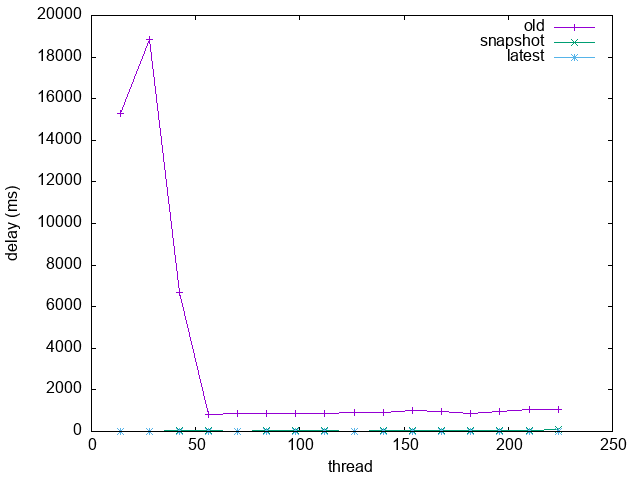
\includegraphics[width=15cm]{data/stable/ycsb-a/news/opposite-delay}
\caption{opposite\_writeフラグを有効にした場合}
\label{fig:a-opposite-delay}
\end{figure}

\begin{figure}[h] 
\centering
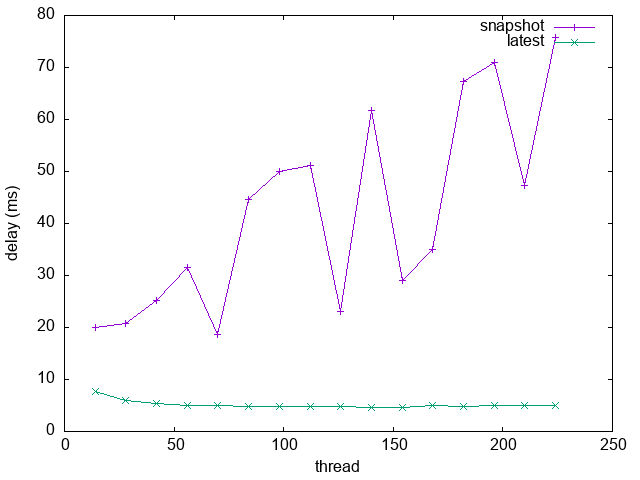
\includegraphics[width=15cm]{data/stable/ycsb-a/news/opposite-delay2}
\caption{opposite\_writeフラグを有効にした場合 snapshotとlatestのみ}
\label{fig:a-opposite-delay2}
\end{figure}

\begin{figure}[h] 
\centering
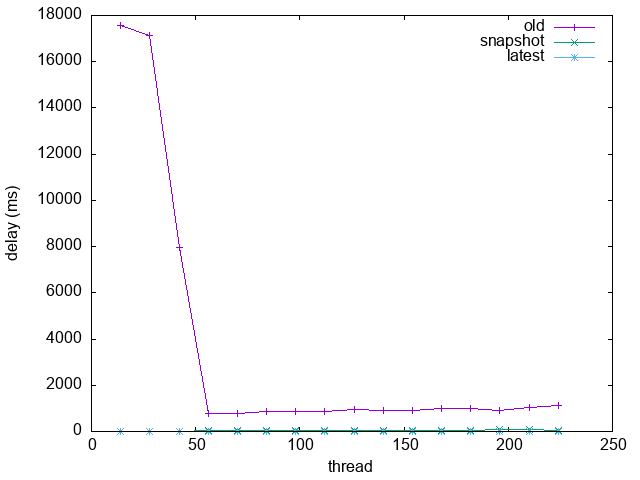
\includegraphics[width=15cm]{data/stable/ycsb-a/news/direct-delay}
\caption{opposite\_writeフラグを無効にした場合}
\label{fig:a-direct-delay}
\end{figure}

\begin{figure}[h] 
\centering
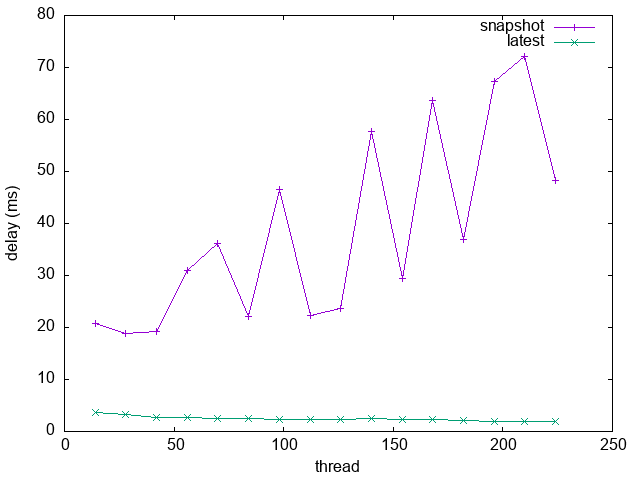
\includegraphics[width=15cm]{data/stable/ycsb-a/news/direct-delay2}
\caption{opposite\_writeフラグを無効にした場合 snapshotとlatestのみ}
\label{fig:a-direct-delay2}
\end{figure}

%TODO oldについてはどう説明する?どっかで平均値の撮り方間違えてる?データ取り直した方がいいんじゃね?逐次実行だから

データの鮮度について図\ref{fig:a-opposite-delay}〜図\ref{fig:a-direct-delay2}に表示した。 

opposite\_writeフラグの有効・無効に関わらず、snapshotよりlatestの方がデータの鮮度が高いことがわかった。これは、セクションほにゃららで説明したように、latestのlookupLatestTransformでは時刻の同期を取ることなく最新の座標変換データを取得するからだと考えられる。

latestについては、opposite\_writeフラグを無効にした方がdelayが小さく、より鮮度の高いデータが取れていることがわかった。これは、先程説明したようにopposite\_writeフラグを無効にすることにより書き込み専用スレッドのabort率が低くなり、書き込みのレイテンシが低下したからだと考えられる。
%TODO 提案手法のとこ

\begin{figure}[h] 
\centering
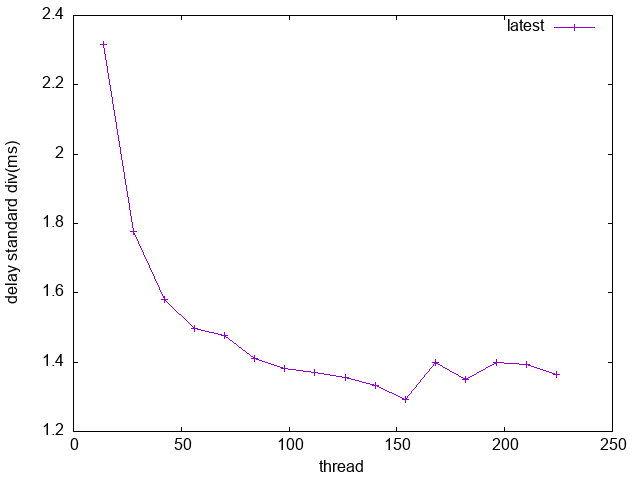
\includegraphics[width=15cm]{data/stable/ycsb-a/news/opposite-stddiv}
\caption{opposite\_writeフラグを有効にした場合}
\label{fig:a-opposite-stddiv}
\end{figure}

\begin{figure}[h] 
\centering
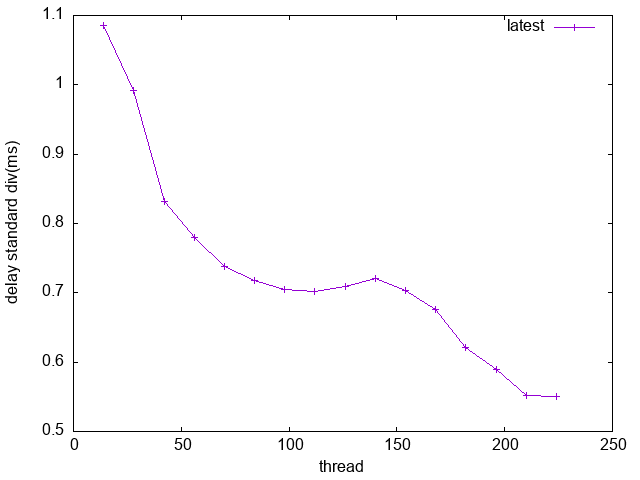
\includegraphics[width=15cm]{data/stable/ycsb-a/news/direct-stddiv}
\caption{opposite\_writeフラグを無効にした場合}
\label{fig:a-direct-stddiv}
\end{figure}


データの同期性について図\ref{fig:a-opposite-stddiv}、図\ref{fig:a-direct-stddiv}に表示した。これらを比較してわかるように、opposite\_writeフラグを無効にした方が全体的に書き込みのタイミングの標準偏差が1/2倍程度になっていることがわかった。これは、先程説明したようにopposite\_writeフラグを無効にすることにより書き込み専用スレッドのabort率が低くなり、書き込みのレイテンシが低下したからだと考えられる。

%\section{YCSB-B}
%read latencyにここまでの差が生じ始めたのはなぜ????明らかにwriteに邪魔されている
%writeスレッドが少ない方がlockの取得率高い?でもabortが多くなっている
%でもwriteのスループットは高い。
%readのレイテンシは悪化している。readがたくさん、writeが少数の特殊な状況においてreadが邪魔
%
%writeのレイテンシは0.5より低い。これはwriteが少ないから。
%でもabortはあまり変わらない。
%
%compare with a
%writeスループットは変わらない
%delayも変わらない
%read latencyは二倍
%read スループットは変わらない
%write latencyは0.1倍
%連続性がないことが一番の問題。
%
%compare with c
%read スループットは1/5
%read レイテンシは10倍


%TODO YCSB-Bについてはひとまずあとで

\section{制御周期}

\begin{figure}[h] 
\centering
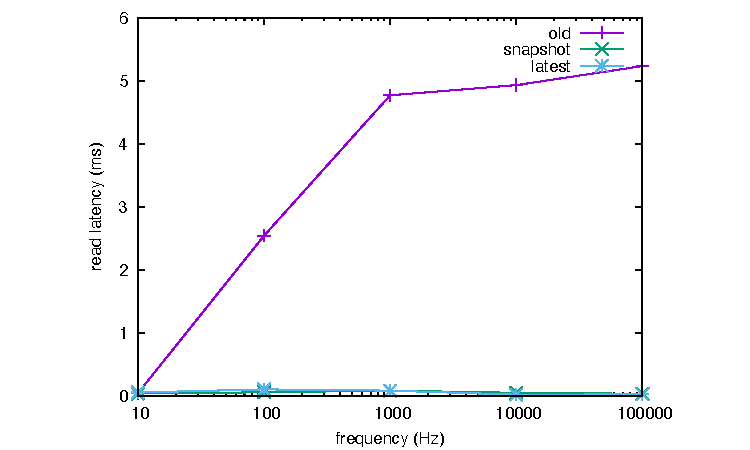
\includegraphics[width=15cm]{latency-frequency}
\caption{制御周期とレイテンシ}
\label{fig:latency-frequency}
\end{figure}



図\ref{fig:latency-frequency}は、スレッド数200の状態でfrequencyを100から100000まで変化させた時の読み込みレイテンシを表している。frequencyを上げるとレイテンシも増えることがわかる。これは、制御周期を増やすことにより並行に実行される操作が増え、スレッド間の競合が増加するからだと考えられる。

%\begin{figure}[h] 
%\centering
%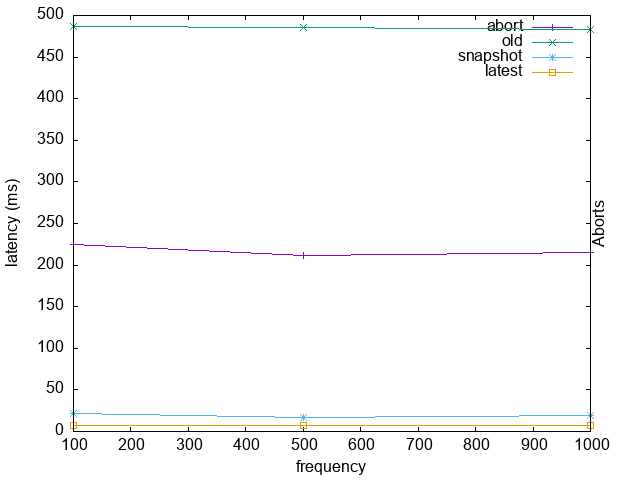
\includegraphics[width=15cm]{frequency-real}
%\caption{制御周期とレイテンシ}
%\label{fig:frequency-real}
%\end{figure}

%TODO 今のままだと問題になる具体的なワークロードを示す

%oldにおいてレイテンシが問題となるワークロードを示したのが図\ref{fig:frequency-real}である。これは、thread=200、joint=1000000、read\_ratio=0.5、read\_len=10000、write\_len=10000におけるレイテンシを表している。
%
%frequencyは100なのでかなり現実的
%snapshotとlatestでは20ms、12msなのに対し、oldでは608msとなり現実的なワークロードでは問題となる。
%ここはjoint数を増やした時のレイテンシの変化を記録する?
%
%この説明は本当にいるのか?
%ヘビ型ロボットや、センサで認識した物体をTFに登録するようなワークロードでは問題となる。
%その場合には、どんなオブジェクトがどこにあるかを統一的に扱う枠組みが必要だろう。例えば今は
%でもその情報は一つのマップには集約されていない。別々のプロセスが別々のデータ型でpublishし、内部の情報はopenではない。
%例えば障害物はmove\_baseによるcostmap、信号はカメラによるYOLO、人や車の検知はLiDARのPointNetのようにデータが分散しており、今は一つにまとまってない!

\chapter{結論}

本研究ではTFライブラリにデータベースの並行性制御技術を導入することにより、マルチコアの性能を活かせ、優れた応答性能をもち、さらにデータの鮮度も向上させることができる事を示した。また、並行性制御技術を導入することにより、今までは実現できなかった新たな操作を提供した。

本研究のようにロボットにおいてデータベースの並行性制御技術を導入する研究アプローチは他になく、ロボットの高性能化のためには並行性制御技術の導入が必要である事を示した。

\chapter{今後の課題}
本研究ではTFライブラリの森構造は変化しないと仮定したが、実際には時間とともにフレームが追加・削除され、またフレーム間の親子関係が変わることがある。例えば、カメラにて認識した物体をTFに登録する場合には森構造へのフレームの追加が頻繁に発生する。データベースの並行性制御技術においてはこのような要素の追加・削除はIDMモデルで扱われ、高度な並行性制御にはphantom anomalyを避ける必要がある。要素の追加・削除についても扱うことが今後の課題である。

本研究では並行性制御の具体的なアルゴリズムとしては2PLを実装したが、Siloを実装した場合の性能比較も行うことが今後の課題である。

また、よりロボット向けのワークロードに対応するため、TFに対する操作に優先順位をつけ、優先順位が高い操作をなるべく早く終わらせるために優先順位キューを実装することも検討が必要である。

ロボットに並行性制御技術を導入する対象として本研究ではTFライブラリを取り上げたが、他にもROSで頻繁に使用されるmove\_baseなどのパッケージにおいても並行性制御技術の導入の検討が必要である。

\chapter*{謝辞}
\addcontentsline{toc}{chapter}{\numberline{}謝辞}

本研究を進めるにあたり、慶應義塾大学准教授川島英之先生、筑波大学システム情報系情報工学域大矢晃久、筑波大学システム情報系情報工学域萬礼応先生に頂きました優れた御指導により、私の研究はとても有意義で満ち足りたものとなりました。また、慶應義塾大学川島研究会秘書藤川綾様には幾多の手続きを丁寧にサポートして頂き,円滑な出張や書類作成,研究環境整備を行うことができました。この研究に関わっていただいたすべての方に深く感謝を申し上げます。

% 参考文献(References)
\newpage
\addcontentsline{toc}{chapter}{\numberline{}参考文献}
\renewcommand{\bibname}{参考文献}


%% 参考文献に bibtex を使う場合
%\bibliographystyle{junsrt}
%\bibliography{ref}

%% 参考文献を直接ファイルに含めて書く場合
	
\begin{thebibliography}{99}


\bibitem{ros} M. Quigley, K. Conley, B. P. Gerkey, J. Faust, T. Foote, J. Leibs, R. Wheeler, and A. Y. Ng, “Ros: an open-source robot operating system,” in ICRA Workshop on Open Source Software, 2009.

\bibitem{tf} T. Foote, "tf: The transform library," 2013 IEEE Conference on Technologies for Practical Robot Applications (TePRA), 2013, pp. 1-6, doi: 10.1109/TePRA.2013.6556373.

\bibitem{2PL} Philip A. Bernstein and Nathan Goodman, "Concurrency Control in Distributed Database Systems" in ACM Computing Surveys, 1981, pp. 185-221

\bibitem{buffer-core} "BufferCore.h", \url{https://github.com/ros/geometry2/blob/noetic-devel/tf2/include/tf2/buffer_core.h}

\bibitem{gaia} "GAIA platform", \url{https://www.gaiaplatform.io}

\bibitem{ros2} "ROS2", \url{https://docs.ros.org/en/rolling/}

\bibitem{autoware} "Autoware", \url{https://tier4.jp/en/autoware/}

\bibitem{silo} Stephen Tu, Wenting Zheng, Eddie Kohler †, Barbara Liskov,
and Samuel Madden. Speedy transactions in multicore in-memory
databases. In SOSP, pages 18–32. ACM, 2013

\bibitem{Cicada} Hyeontaek Lim, Michael Kaminsky, and David G Andersen. Cicada: Dependably fast multi-core in-memory transactions. InProceedings of the 2017 ACM International Conference onManagement of Data, p. p. 21âĂŞ35, 2017.

\bibitem{ycsb} Brian F Cooper, Adam Silberstein, Erwin Tam, Raghu Ramakrishnan, and Russell Sears. Benchmarking cloud serving systems with ycsb. InProceedings of the 1st ACM symposiumon Cloud computing, p. p. 143âĂŞ154, 2010.

\bibitem{nowait} Guna Prasaad, Alvin Cheung and Dan Suciu. Improving High Contention OLTP Performance via Transaction Scheduling. 


\end{thebibliography}


\end{document}
